\frame{\frametitle{Caso de estudio}
  \begin{itemize}
  \item El caso más simple corresponde a MHD incompresible con un
    campo magnético $\vec{B_0}$ de fondo, para el cual la relación de
    dispersión lineal $\omega = \vec{k}\cdot\vec{V_A}$ describe ondas
    de Alfv\'en, con $\vec{V_A} = \vec{B_0}/\sqrt{4\pi/\rho}$.
  \item Las escalas temporales pertinentes serán el tiempo no
    lineal $\tau_{nl}$ y las asociadas
    con los efectos no lineales dependientes de la escala, el
    \emph{sweeping} no local ($\tau_{sw}$) y la propagación de ondas de Alfvén ($\tau_A$).
  \end{itemize}
}
\note[itemize]{
\item
\item OBJETIVOS
}







%%%%%%%%%%%%%%%%%%% ANTES
%% \frame{\frametitle{Introducción}
%%   \begin{itemize}
%%   \item Al comienzo de los 70's, las investigaciones de turbulencia
%%     hidrodinámica concluyeron que el \emph{sweeping} domina la
%%     descorrelación temporal en el rango inercial.
%%   \item Recientemente, Servidio \emph{et al} (2011) estudiaron el caso
%%     MHD. Concluyeron que, para el caso de turbulencia isotrópica, la
%%     descorrelación temporal en MHD está gobernada por las
%%     interacciones no locales, pero no pudieron distinguir entre los
%%     efectos de \emph{sweeping} y las distorsiones de Alfv\'en.
%%   \end{itemize}
%% }

%\section{Objectives}
\frame{\frametitle{Objetivos}
  \begin{itemize}
  \item Generalizar el estudio hecho por Servidio a plasmas
    magnetizados a grandes escalas, donde vale la aproximación MHD.
  \item Estudiar y entender la descorrelación temporal de las
    fluctuaciones.
  \item De esta manera, poder diferenciar entre los efectos no
    lineales, de \emph{sweeping} y de Alfv\'en.
  \item Clark di Leoni \emph{et al} (2014) propusieron considerar las
    fluctuaciones a más de una escala en un flujo rotante, para
    discernir entre los diferentes fenómenos asociados a la
    descorrelación temporal.
  \end{itemize}
}

%\section{Equations and numerical simulations}
\frame{\frametitle{Las ecuaciones MHD}
  \begin{equation*}\label{eq:MHD_v}
    \frac {\partial {\bf v}}{\partial t} +
    {\bf v }\cdot \nabla {\bf v} = -\frac{1}{\rho}\nabla p +
    {\bf j} \times {\bf B} + \frac{1}{R} \nabla^2{\bf v} + \vec{F}_v
  \end{equation*}
  \begin{equation*}\label{eq:MHD_b}
    \frac{\partial {\bf b}}{\partial t} = \nabla \times ({\bf v} \times {\bf B})
    + \frac{1}{R_m} \nabla^2 {\bf b} + \vec{F}_b
  \end{equation*}
  \begin{itemize}
    \item ${\bf B} = {\bf b} + {\bf B_0}$, con una parte fluctuante ${\bf
        b}$ y un campo medio DC ${\bf B_0}=B_0\hat{x}$
    \item Las unidades se basan en una velocidad característica, la
      velocidad de Alfv\'en de las fluctuaciones del campo magnético,
      $v_0 = \sqrt{\langle b^2 \rangle /(4\pi\rho)}$.
    \item $R$ y $R_m$ son los números de Reynolds cinético y magnético.
    \item La unidad temporal es $t_0 = L/v_0$, el tiempo de cruce
      Alfv\'enico basado en las fluctuaciones de campo magnético.
  \end{itemize}
}
\note[itemize]{
\item Forzados
\item
\item TIEMPOS CARACTERÍSTICOS
}


%\subsection{Characteristic times}
\frame{\frametitle{Tiempos característicos}
\begin{block}{Tiempo no lineal}
  \begin{itemize}
    \item Local eddy turnover.
  \end{itemize}
  \begin{equation*}
    \tau_{nl} \sim \left[ k v(k) \right]^{-1} \Rightarrow \tau_{nl} \approx \left [ v_{rms} L^{-1/3} \left(\sqrt{k^2_\perp + k^2_\parallel}\right)^{2/3}\right ]^{-1}
  \end{equation*}
\end{block}
\begin{block}{Tiempo de \emph{sweeping}}
  \begin{itemize}
    \item Advección de estructuras de pequeña escala por el flujo de gran escala. 
  \end{itemize}
  \begin{equation*}
    \tau_{sw} \approx \left( v_{rms}\sqrt{k^2_\perp + k^2_\parallel} \right)^{-1}
  \end{equation*}
\end{block}
\begin{block}{Tiempo de Alfv\'en}
  \begin{equation*}
    \tau_A \approx \left( B_0 k_\parallel \right)^{-1}
  \end{equation*}
\end{block}
}
\note[itemize]{
\item A partir de las ecuaciones MHD, salen los tiempos característicos
\item Faltan las constanted $C_i \sim 1$
\item
\item FUNCIONES DE CORRELACIÓN
}



%\subsection{Decorrelation function}
\frame{\frametitle{Función de correlación}
  \begin{itemize}
  \item La estadística de un campo (por ej, el magnético) puede ser
    caracterizada por la función de autocorrelación espacio-temporal a
    dos puntos, $R(\vec{r},\tau) = \left\langle \vec{b}(\vec{x},t)
    \cdot \vec{b}(\vec{x}+\vec{r},t+\tau) \right\rangle / \left\langle
    \vec{b}^2 \right\rangle$
  \item Transformando Fourier en $r$ conduce a una densidad espectral
    temporalmente retrasada $S(\vec{k}, \tau) =
    S(\vec{k})\Gamma(\vec{k},\tau)$
  \item $\Gamma(\vec{k},\tau)$ representa los efectos dinámicos de
    descorrelación que describen la descorrelación de tiempo de cada
    modo espacial $\vec{k}$.
  \item $\Gamma(\vec{k},\tau)$ es la función de correlación temporal
    para $\vec{k}$.
  \item En presencia de un campo guía, $\Gamma = \Gamma(\vec{k}_\perp,
    \vec{k}_\parallel, \tau)$ ayuda a entender la dinámica en
    distintas regiones del espacio de Fourier.
  \end{itemize}
}
\note[itemize]{
\item 5) Esto nos da información acerca de cómo la memoria en una
    dirección afecta a la otra, y de cómo podemos distinguir entre el
    \emph{sweeping} aleatorio y la propagación de Alfv\'en.
\item
\item SIMULACIONES
}



%\subsection{Numerical simulations}
\frame{\frametitle{Simulaciones numéricas}
  \begin{itemize}
    \item Código pseudoespectral estándar que resuelve numéricamente
      las ecuaciones 3D-MHD con un campo guía.
    \item Runge-Kutta de segundo orden como esquema de integración temporal.
    \item \emph{Aliasing} removido con el método de truncamiento de la
      regla de los dos-tercios.
    \item Condiciones de contorno periódicas.
    \item Tamaño de la caja de $2\pi L$, donde $L=1$ es la longitud de
      correlación inicial de todas las fluctuaciones.
    \item $N^3 = 512^3$ puntos de grilla..
    \item $B_0 = 0$, $0.25$, $1$, $4$ y $8$, en unidades del valor
      \emph{rms} inicial de las fluctuaciones magnéticas.
    \item Forzado en la banda $0.9 \leq k \leq 1.8$, con componentes
      aleatorias y temporalmente coherentes ($\tau_f \sim 1$).
  \end{itemize}
}
\note[itemize]{
\item Sakura. 9 nodos 224 clusters.
\item Tardan $\sim 1$ mes.
\item Pesan 1GB
}


%\section{Results}
%\subsection{Energy spectra and dominant time scales}
\frame{\frametitle{Algunos resultados obtenidos...}
  
}


\frame{\frametitle{Espectros de energía y escalas de tiempo dominantes}
  Espectros energéticos perpendiculares reducidos
  \begin{center}
    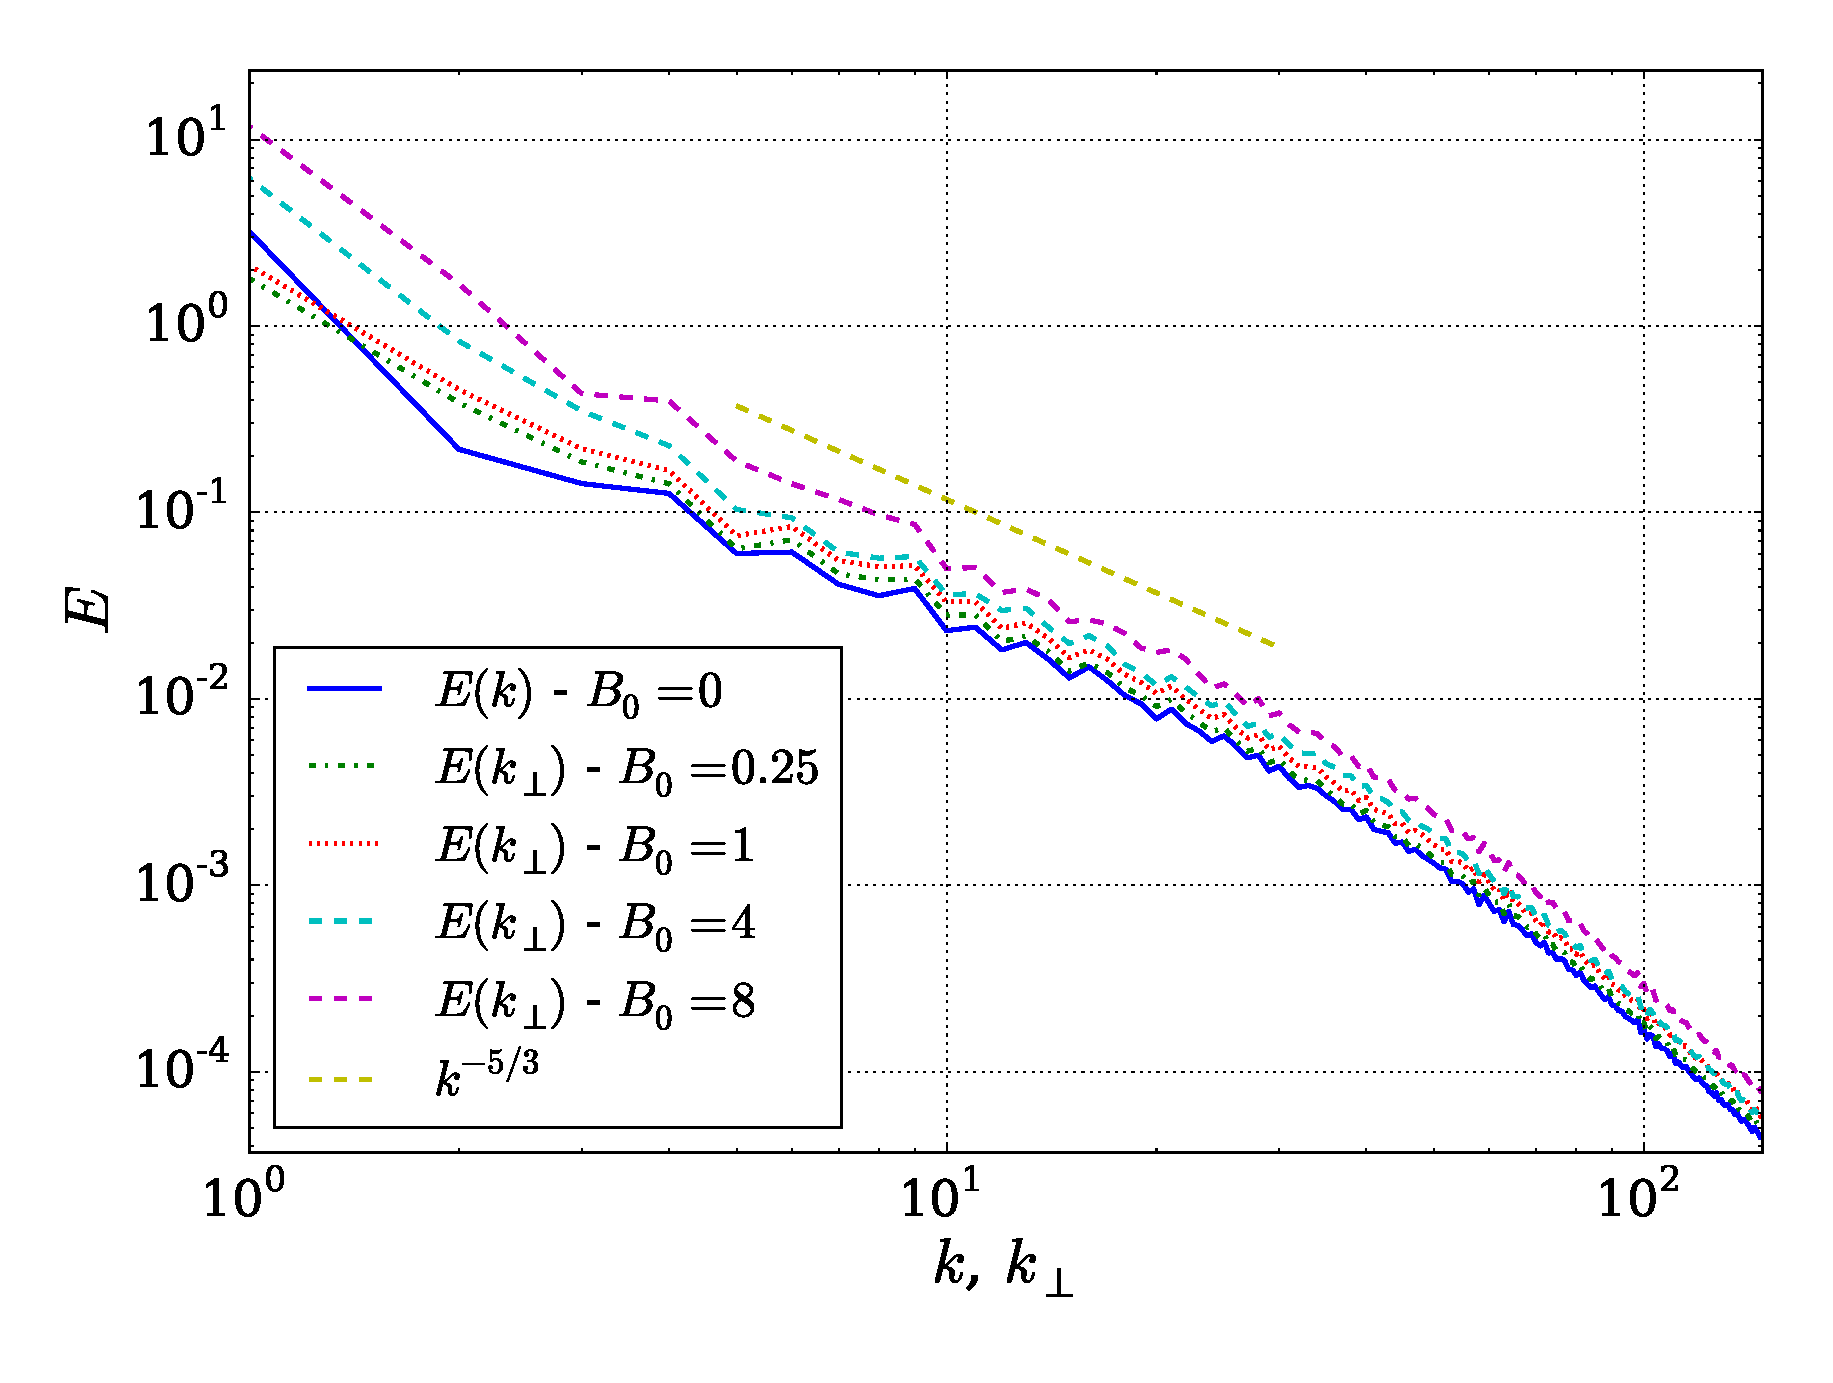
\includegraphics[width=0.7\columnwidth]{P1/fig1_E.eps}
  \end{center}
}
\note[itemize]{
\item Es, básicamente, la energía en función de $k_\perp$.
\item
\item Espectro energético perpendicular reducido y promediado
  temporalmente: $E\left(k_\perp\right) = \frac{1}{T}\int\int
  e(|\vec{k_\perp}|, k_\parallel, t) \, dk_\parallel~dt$
\item Se calcula a partir del espectro axisimétrico.
\item
\item ESPECTRO AXISIMÉTRICO. ENERGÍA EN FUNC DE KPARA Y KPERP

}


\frame{\frametitle{Espectros de energía y escalas de tiempo dominantes}
  \underline{Isocontornos del espectro axisimétrico de energía}
  \pause
  {\Large : $B_0 = 0$}\\
  \begin{center}
    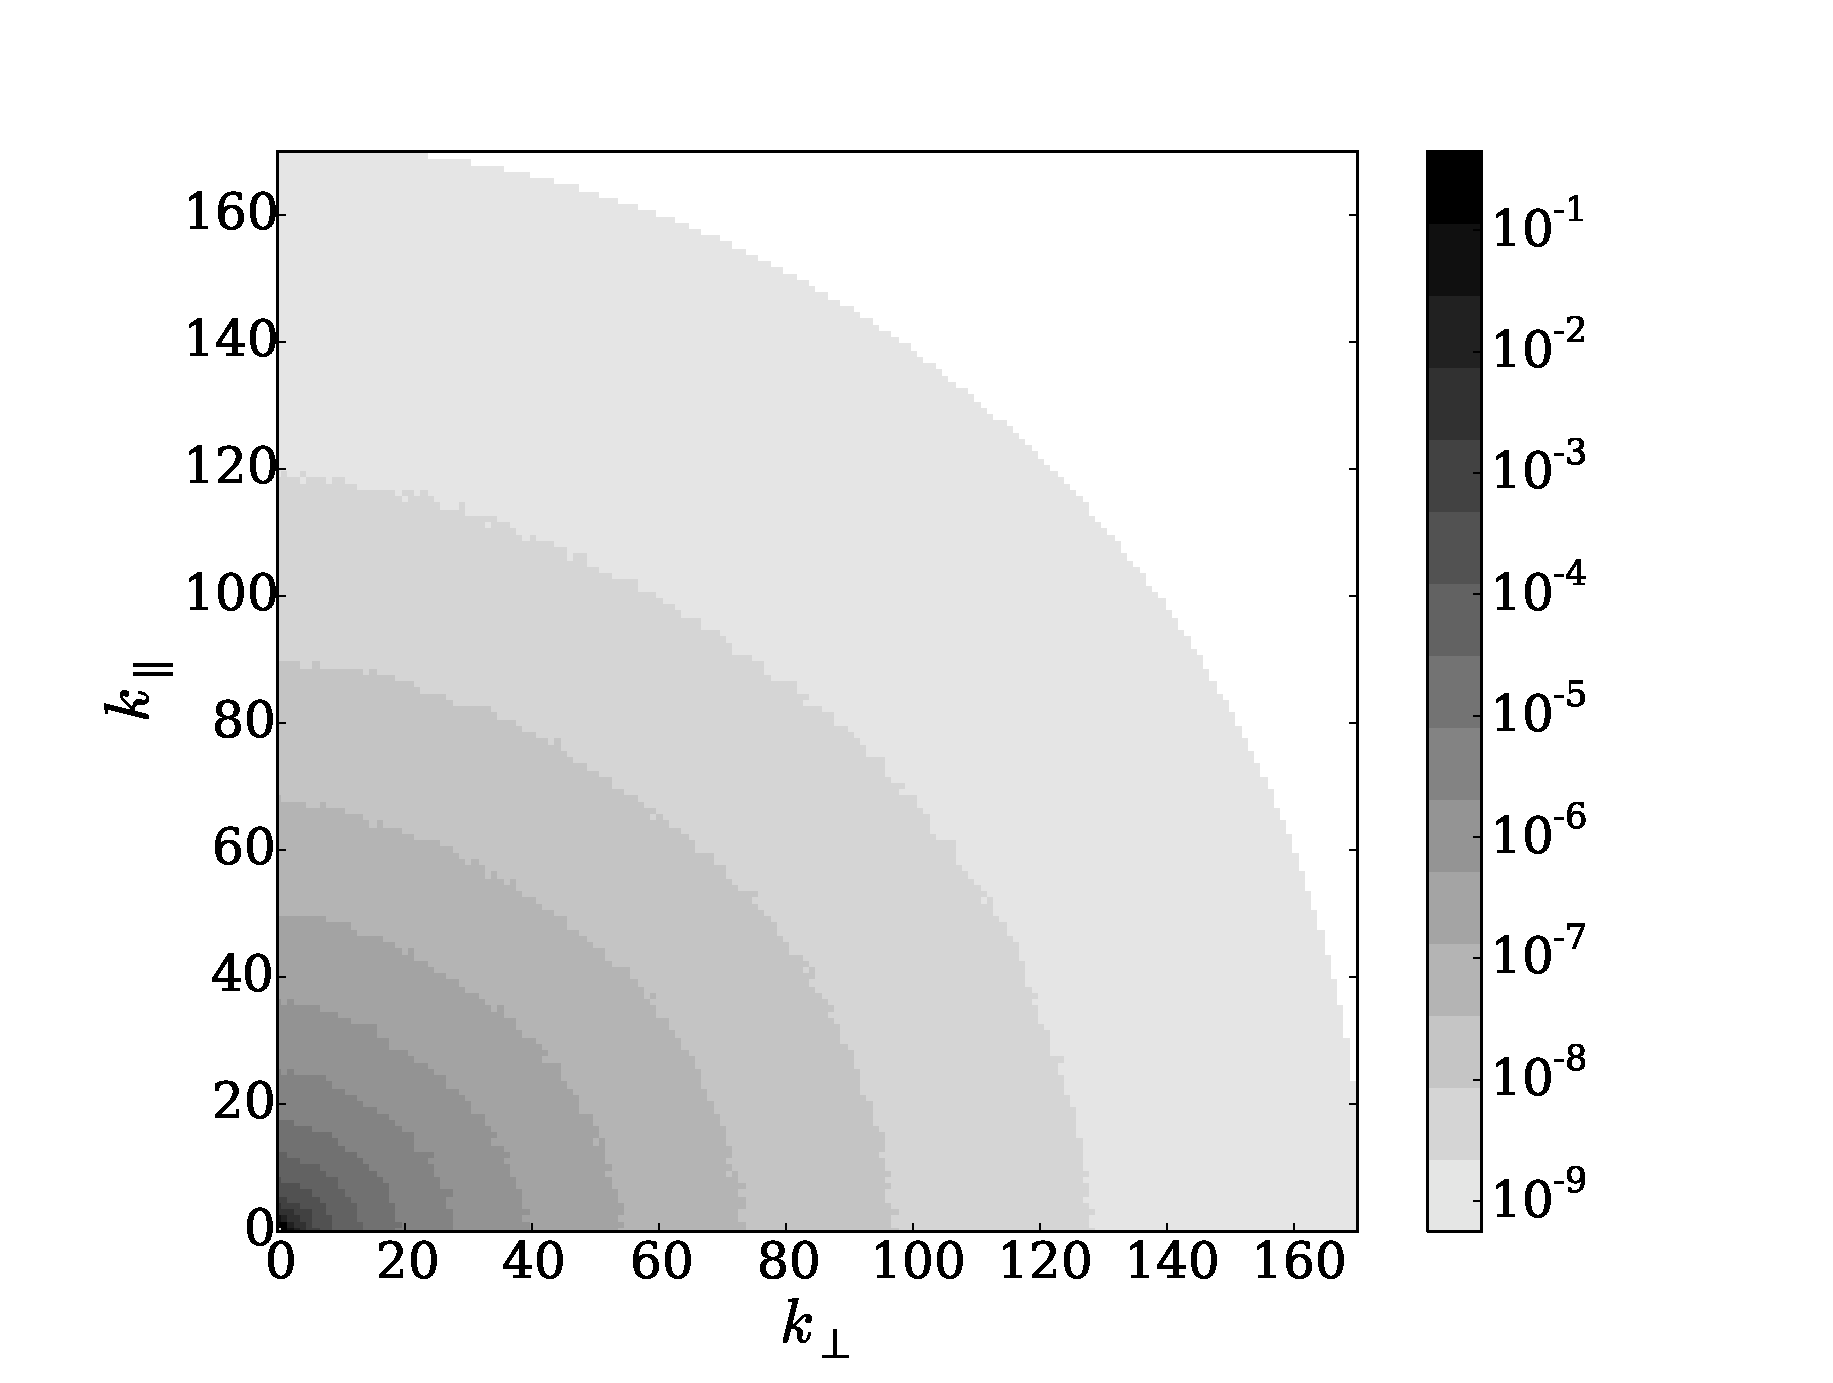
\includegraphics[width=0.7\columnwidth]{P1/fig2_B0.eps}
  \end{center}
}
\note[itemize]{
\item El espectro axisimétrico de energía $e(|\vec{k_\perp}| =
  \sqrt{k_y^2+k_z^2}, k_\parallel = k_x, t)$.
\item Para $B_0 = 0$, los contornos son círculos, como se esperaba.
}



\frame{\frametitle{Espectros de energía y escalas de tiempo dominantes}
  \underline{Isocontornos del espectro axisimétrico de energía}
  { : $B_0 = 1$}\\
  \begin{center}
    \includegraphics[width=0.7\columnwidth]{P1/fig2_B1_explanation.eps}
  \end{center}
}
\note[itemize]{
\item Aumenta $B_0$, mayor E concentrada cerca de $k_\parallel=0$
\item Formación de estructuras elongadas en la dirección del campo guía
\item
\item o, en otras palabras, del
  relativo decrecimiento de los gradientes paralelos del campo con
  respecto a los gradientes perpendiculares).
\item
\item La región con $\tau_{nl} \leq \tau_{sw}$ es un círculo pequeño
  alrededor del origen.
}




\frame{\frametitle{Espectros de energía y escalas de tiempo dominantes}
  {\underline{Isocontornos del espectro axisimétrico de energía}}\\ \vspace{1cm}
  \begin{columns}
    \column{0.5\textwidth}
    \begin{minipage}[t]{1\textwidth}
      \begin{center} 
        {$B_0 = 0.25$}\\
        \includegraphics[width=\columnwidth]{P1/fig2_B025.eps}
      \end{center}
    \end{minipage}
    \column{0.5\textwidth}
    \begin{minipage}[t]{1\textwidth}
      \begin{center}
        {$B_0 = 8$}\\
        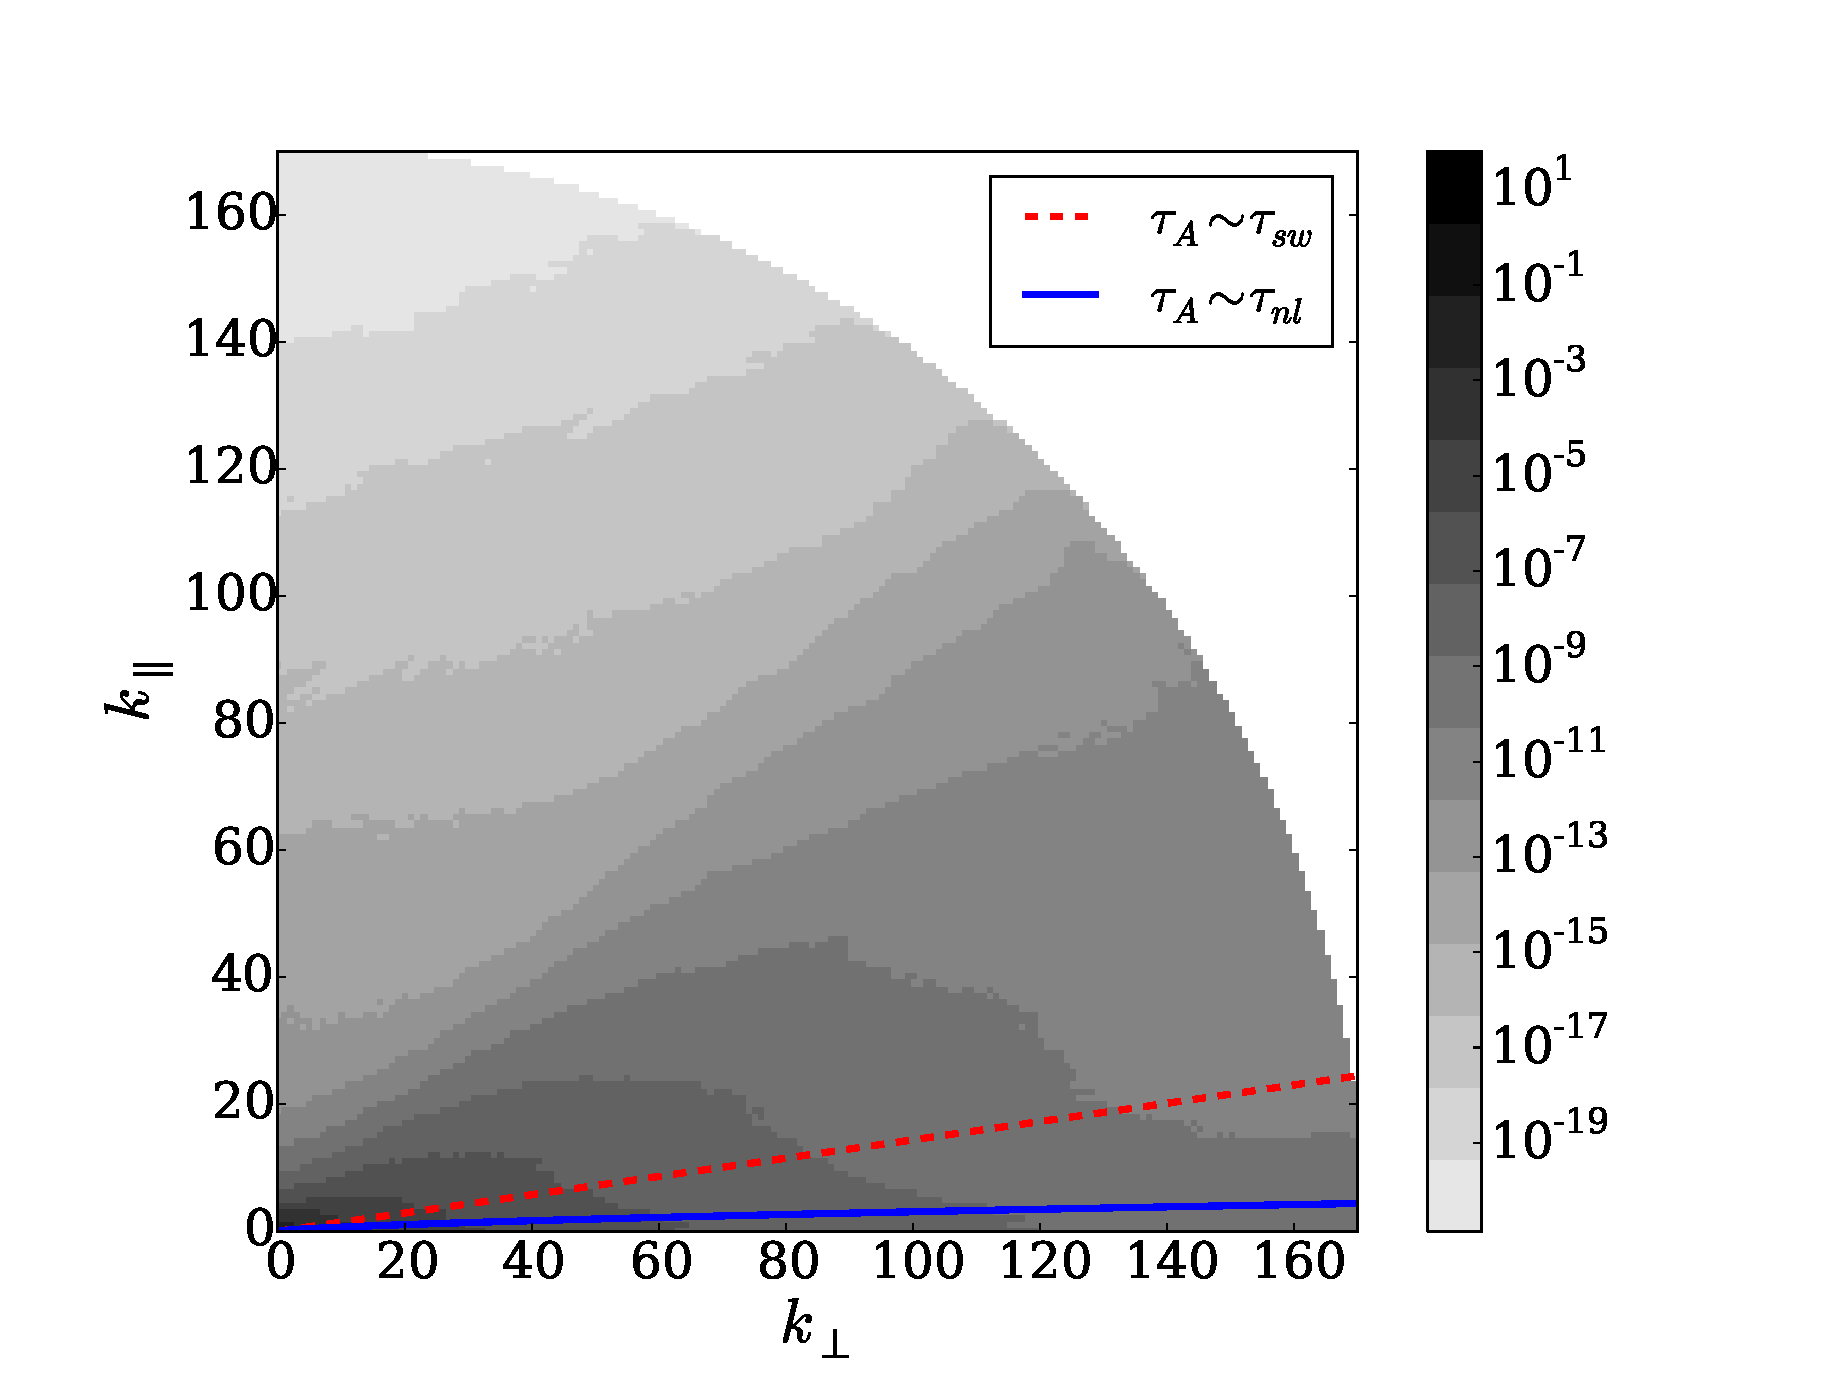
\includegraphics[width=\columnwidth]{P1/fig2_B8.eps}
      \end{center}
    \end{minipage}
  \end{columns}
}
\note[itemize]{
\item Para $B_0 = 0.25$, el tiempo de \emph{sweeping} es el más rápido
  en todos los casos..
\item Para $B_0 = 8$, mayoría de modos con tiempo de Alfvén como el
  más rápido, pero mucha energía fuera de estos modos.
}



%\subsection{Spatio-temporal spectra}
\frame{\frametitle{Espectros espacio-temporales}
  {\underline{Espectro energético normalizado $E({\bf k}, \omega)/E({\bf k})$}}
  \pause
  { : $B_0=0.25$}
  \begin{center}
    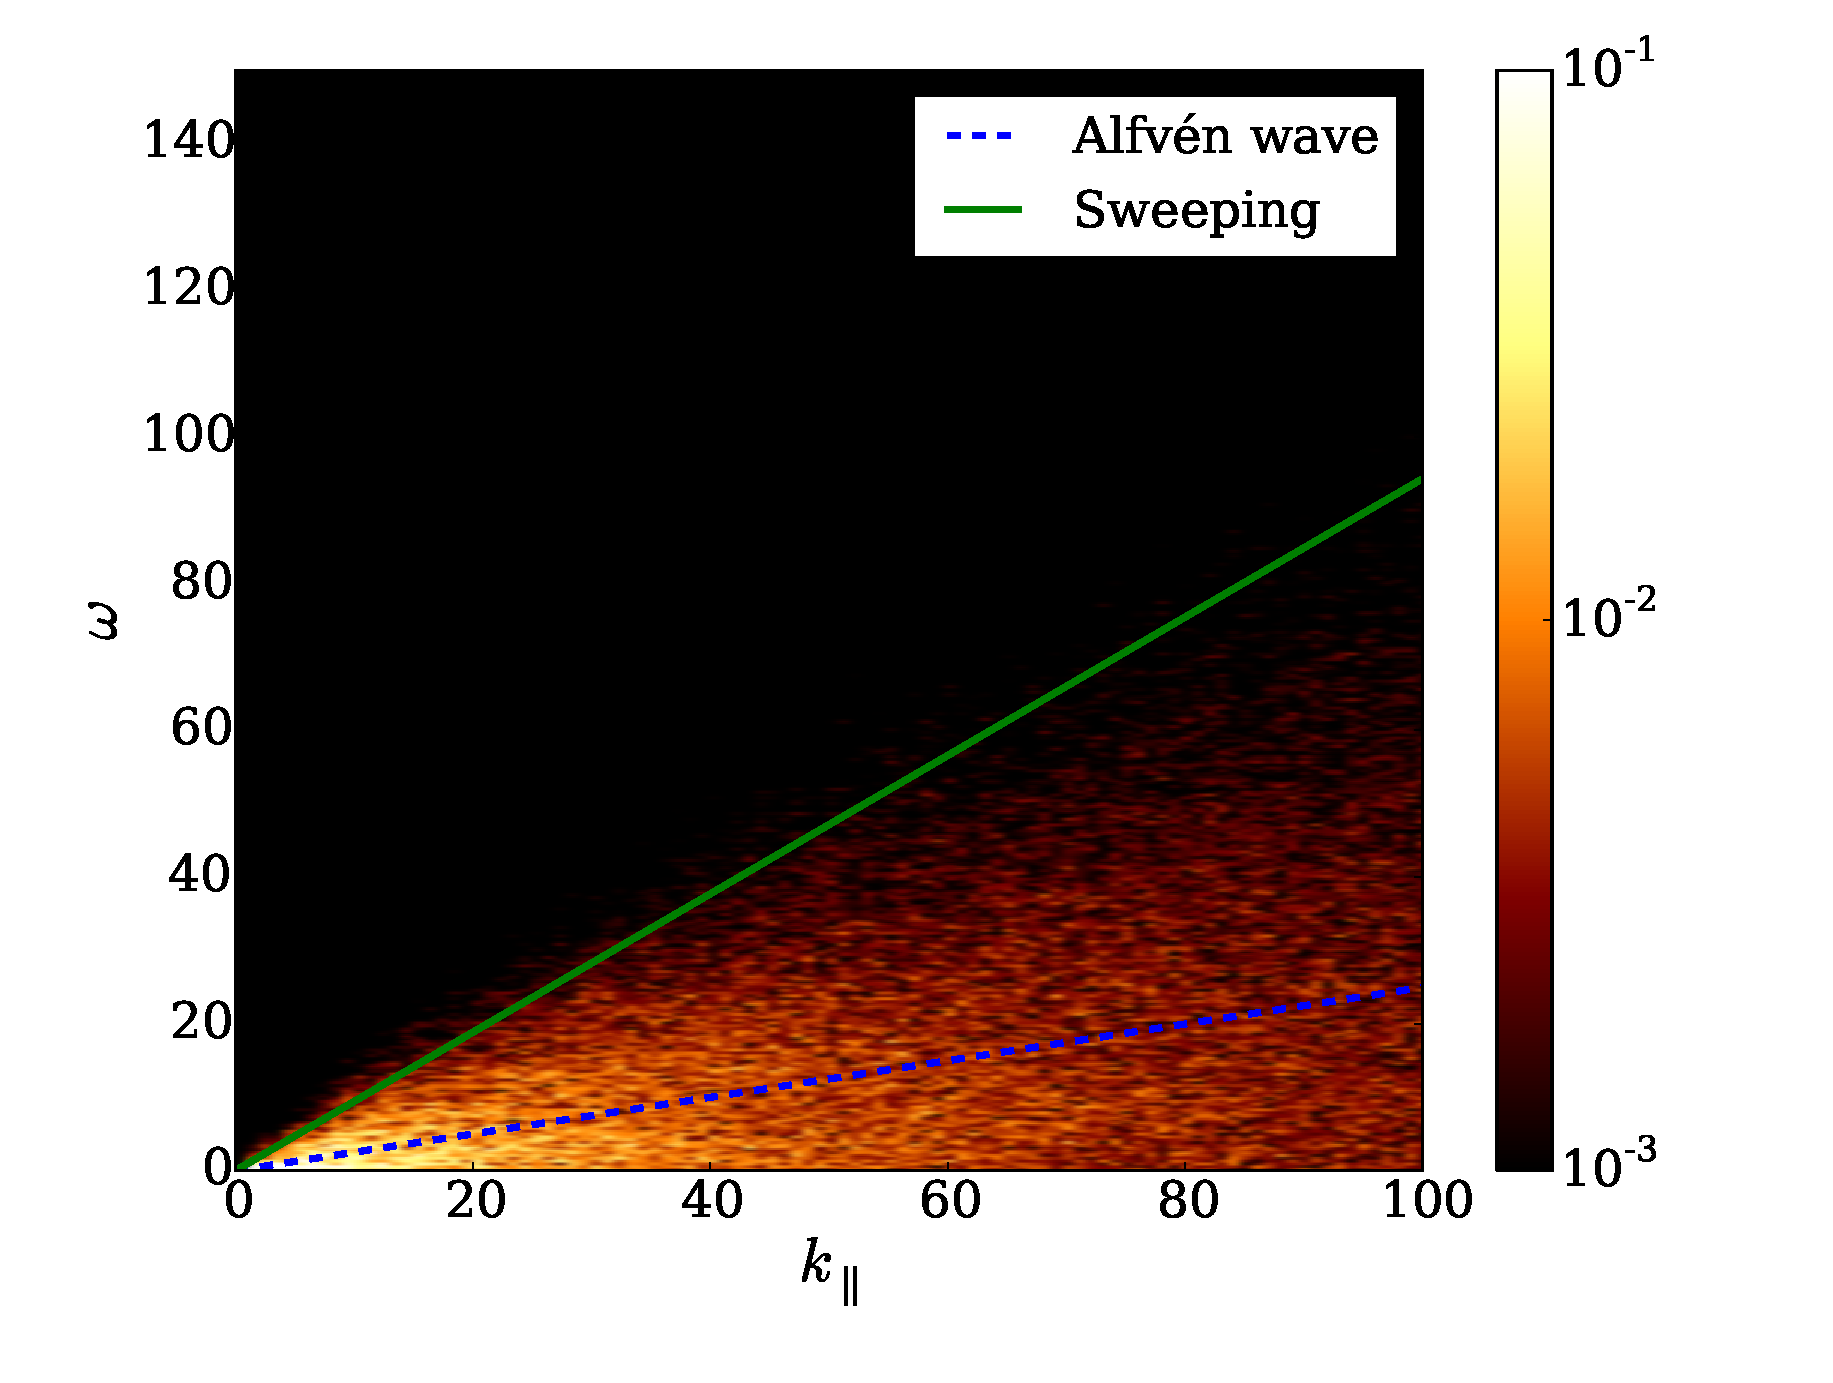
\includegraphics[width=0.7\columnwidth]{P1/fig3_B025_Etot.eps}
  \end{center}
}
\note[itemize]{
\item $k_\perp=0$ fijo. Líneas de \emph{sweeping} y Alfvén.
\item Regiones claras: mayor densidad energética.
\item Espectro: Fourier en $t$ y $r$ de $\vec{z}^\pm$. Acumulación de
  energía: dominio de un efecto físico (i.e., de su frecuencia
  asociada) en la dinámica del plasma a una dada escala $\sim
  1/k_\parallel$.
\item Para $B_0 = 0.25$, dispersión de energía por debajo de la línea
  de \emph{sweeping}. Excitación en modos con frecuencias iguales o
  menores que $\omega = v_{rms} k_\parallel$, indicando que las
  estructuras de escalas pequeñas están siendo advectadas por todas
  las velocidades iguales o menores a $v_{rms}$ $\Rightarrow$ embudo.
\item Pequeña acumulación cerca de la dispersión de Alfvén para
  $k_\parallel$ pequeños.
}



\frame{\frametitle{Espectros espacio-temporales}
  {\underline{Espectro energético normalizado $E({\bf k}, \omega)/E({\bf k})$} : $B_0=1$}
  \begin{center}
    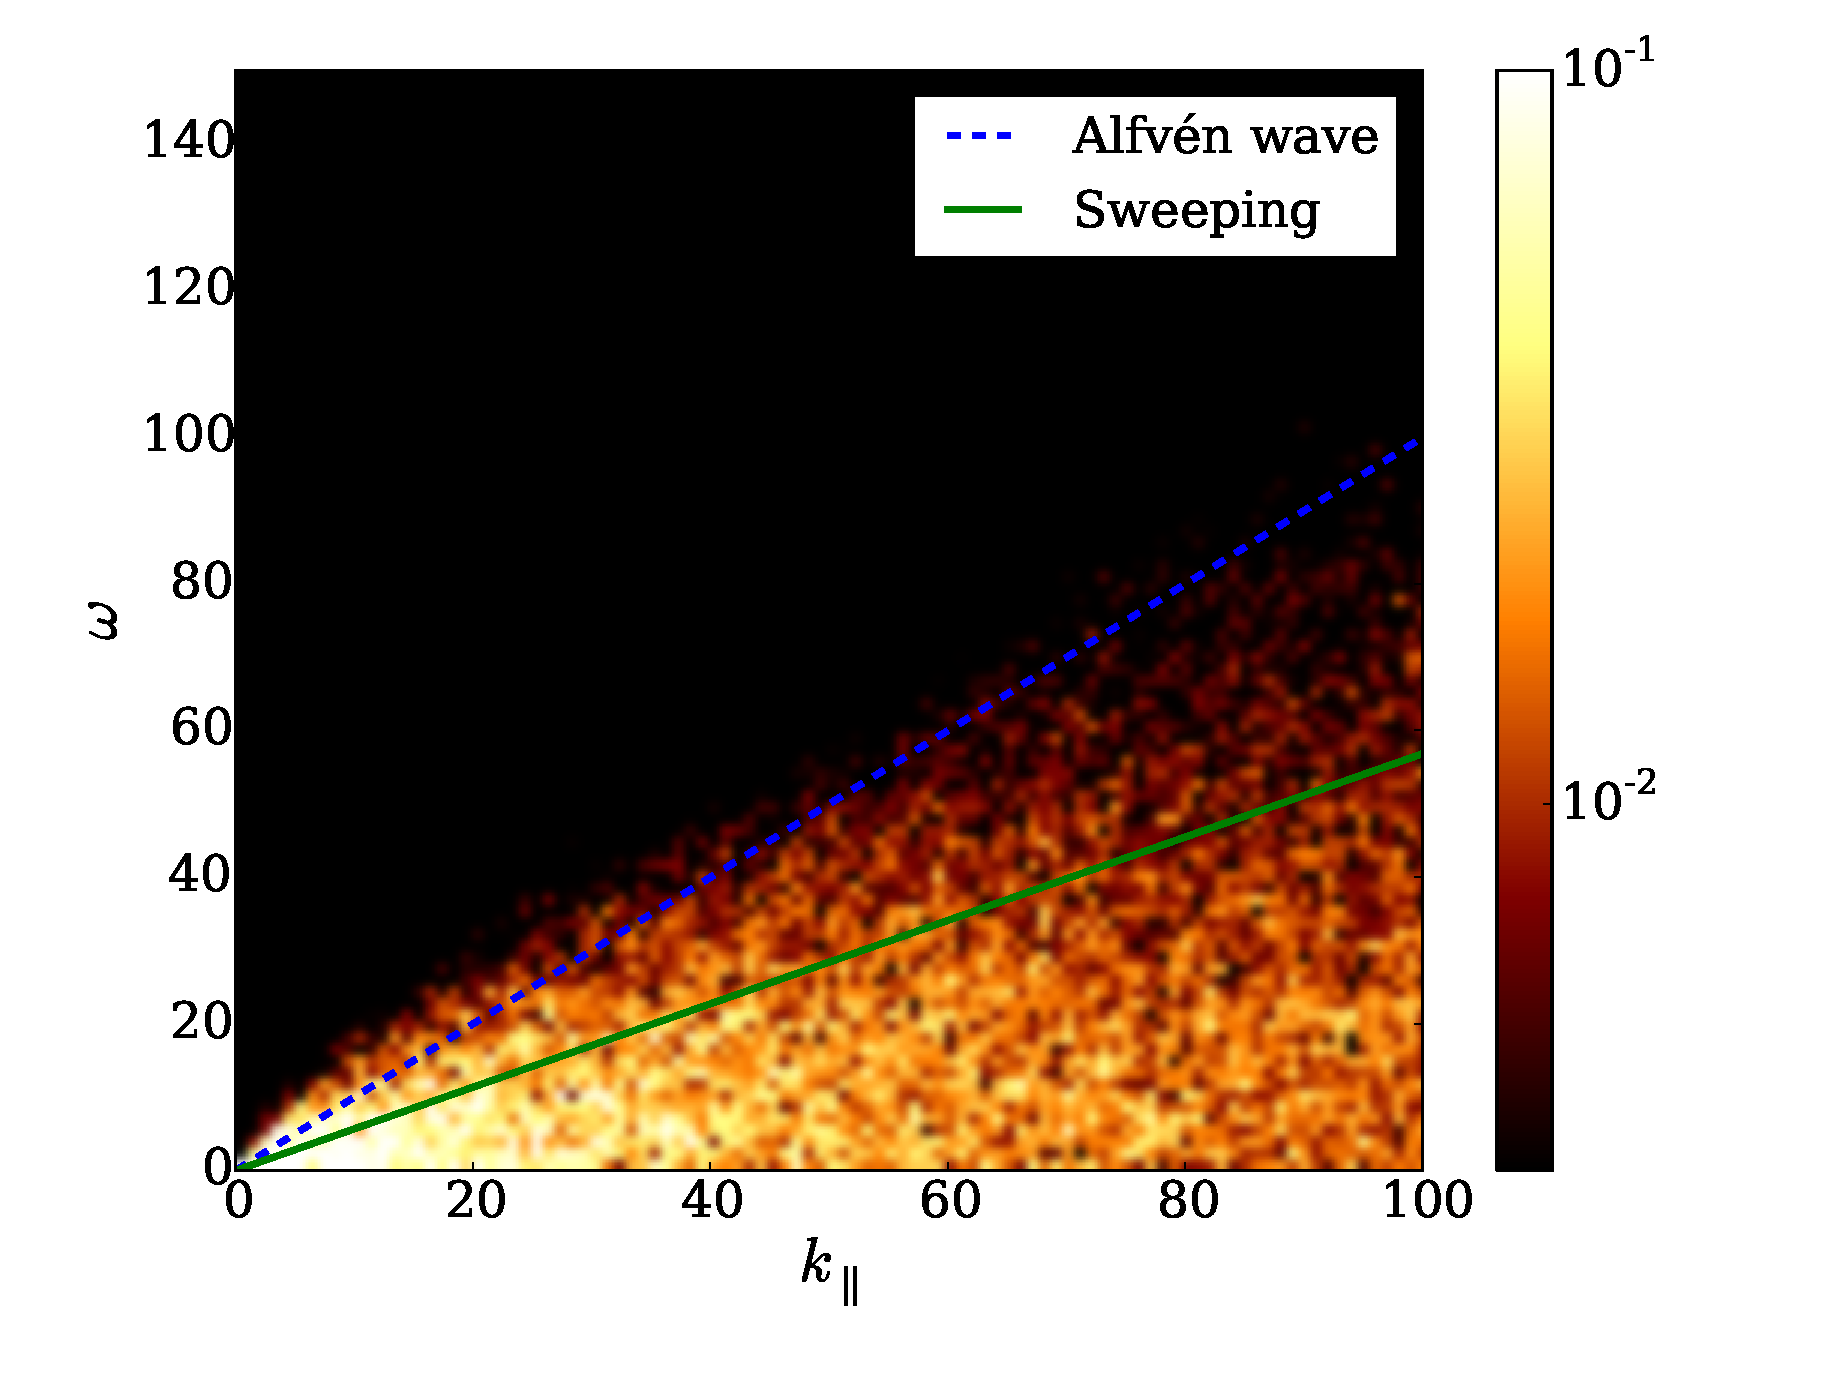
\includegraphics[width=0.7\columnwidth]{P1/fig3_B1_Etot.eps}
  \end{center}
}
\note[itemize]{
\item $B_0=1$, parte de E por encima de \textit{sweeping}, y siguiendo la relación de
  dispersión de Alfvén.
\item Igualmente, espectro amplio, con mucha energía en embudo.
}



\frame{\frametitle{Espectros espacio-temporales}
  {\underline{Espectro energético normalizado $E({\bf k}, \omega)/E({\bf k})$} : $B_0=8$}
  \begin{center}
    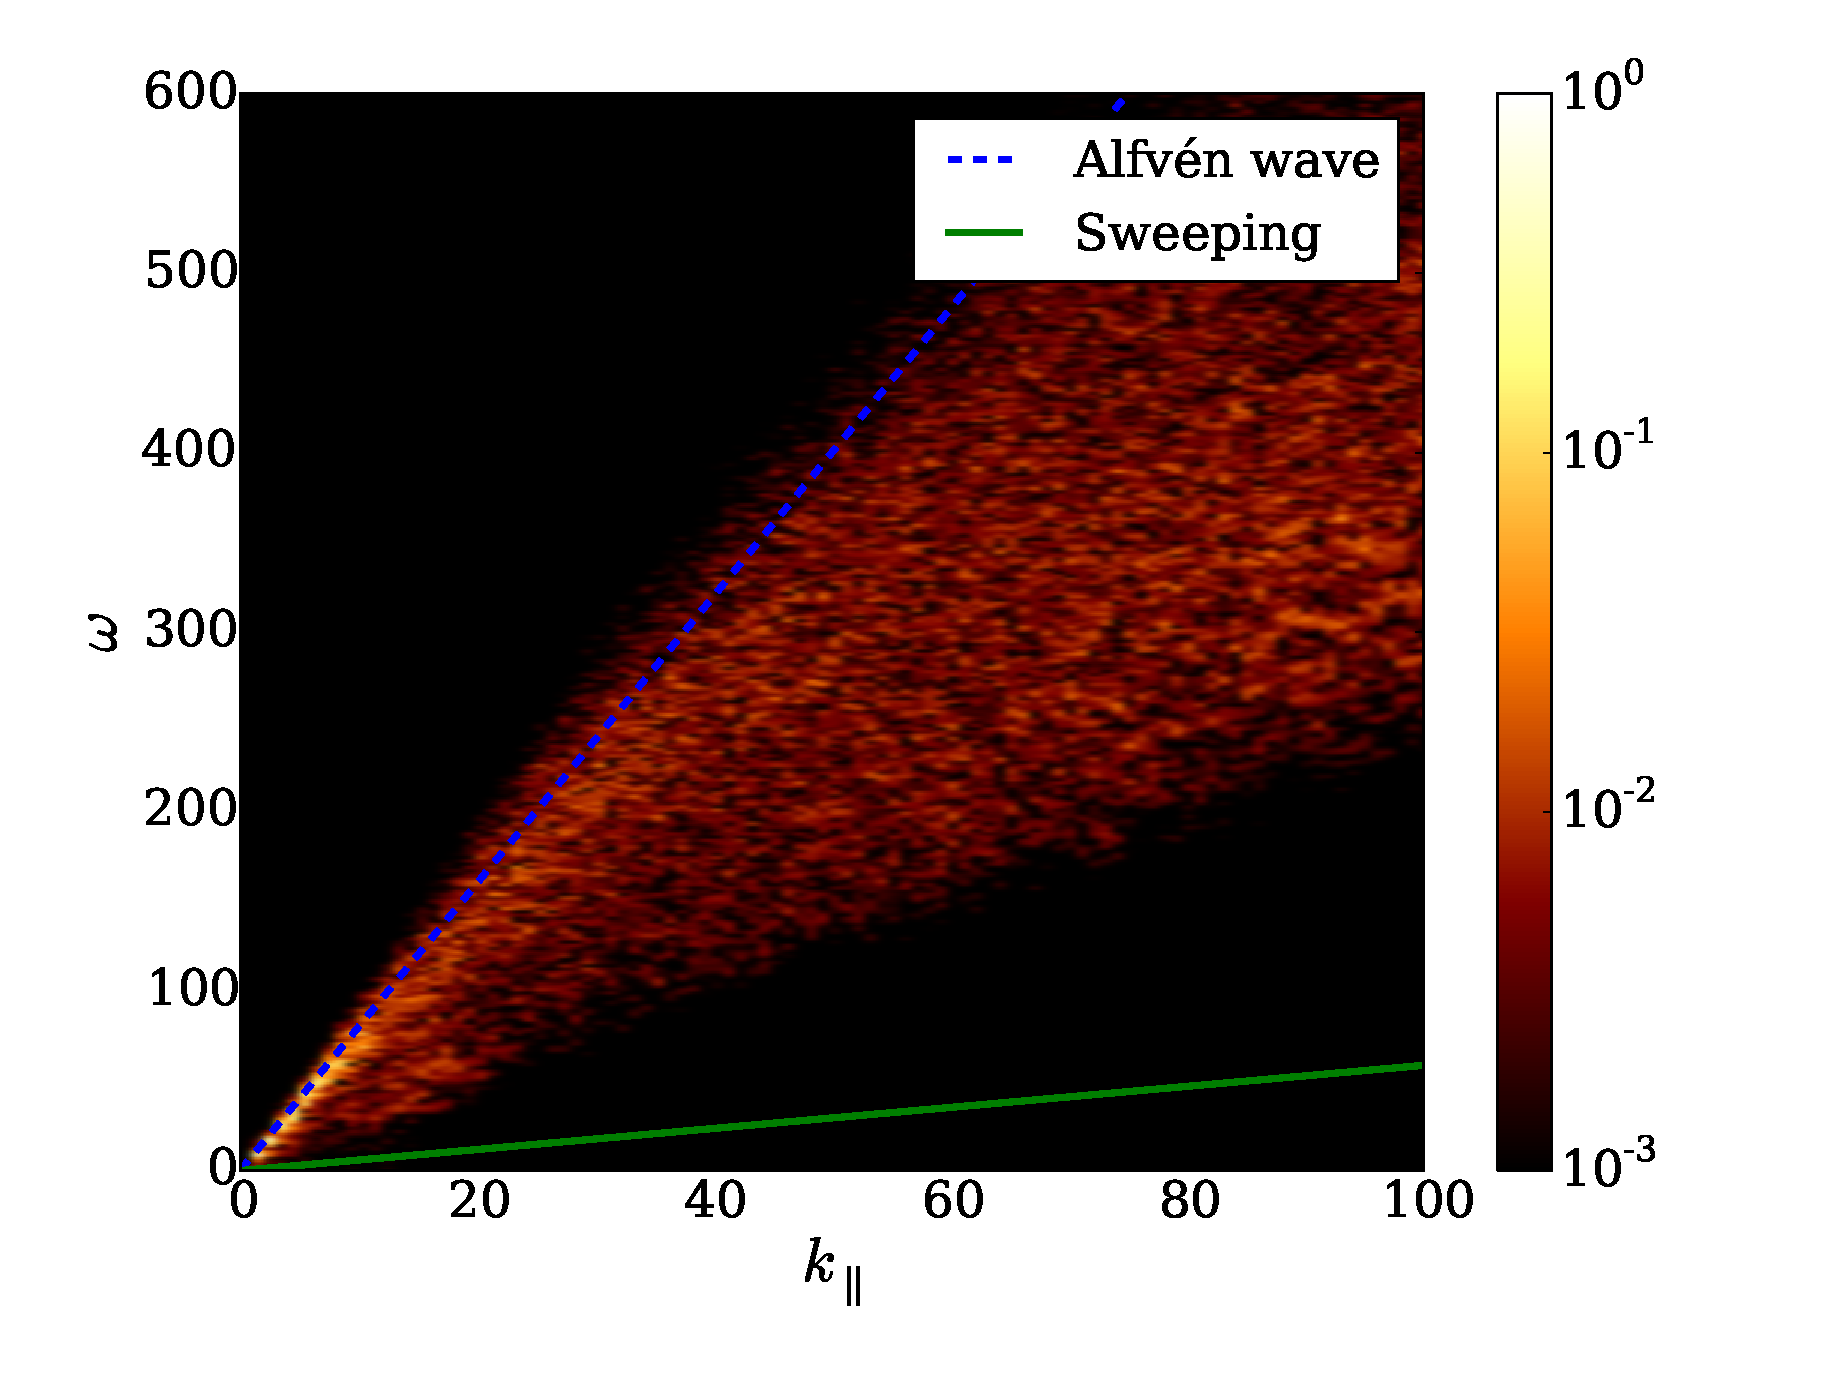
\includegraphics[width=0.7\columnwidth]{P1/fig3_B8_Etot.eps}
  \end{center}
}
\note[itemize]{
\item $B_0=8$, E alrededor de Alfvén, ppalmente hasta $k_\parallel \approx 10$.
\item Luego, se dispersa hacia \textit{sweeping}.
\item Este comportamiento indica una competición entre el tiempo de
  \textit{sweeping} y el tiempo de Alfvén, con este último resultando
  dominante a grandes escalas para valores de $B_0$ grandes.
\item Meyrand (2016): transición de un
  espectro ondular estrecho a un espectro más amplio, aunque la escala
  y el mecanismo responsable para esta transición no fue
  estudiado. Como confirmaremos posteriormente, la competencia entre
  los tiempos de \textit{sweeping} y de Alfvén como el tiempo de
  descorrelación dominante es la responsable del cambio observado en
  el comportamiento del espectro.
 }




%\subsection{Correlation functions and decorrelation time}
\frame{\frametitle{Funciones de correlación: $\Gamma(k_\perp,k_\parallel,\tau)$}
  \pause
  Caso con $B_0 = 1$\vspace{10pt}
  \begin{columns}
    \column{0.5\textwidth}
    \begin{minipage}[t]{1\textwidth}
      \begin{center} 
        $\Gamma(k_\perp=0,k_\parallel=k_0,\tau)$ \\
        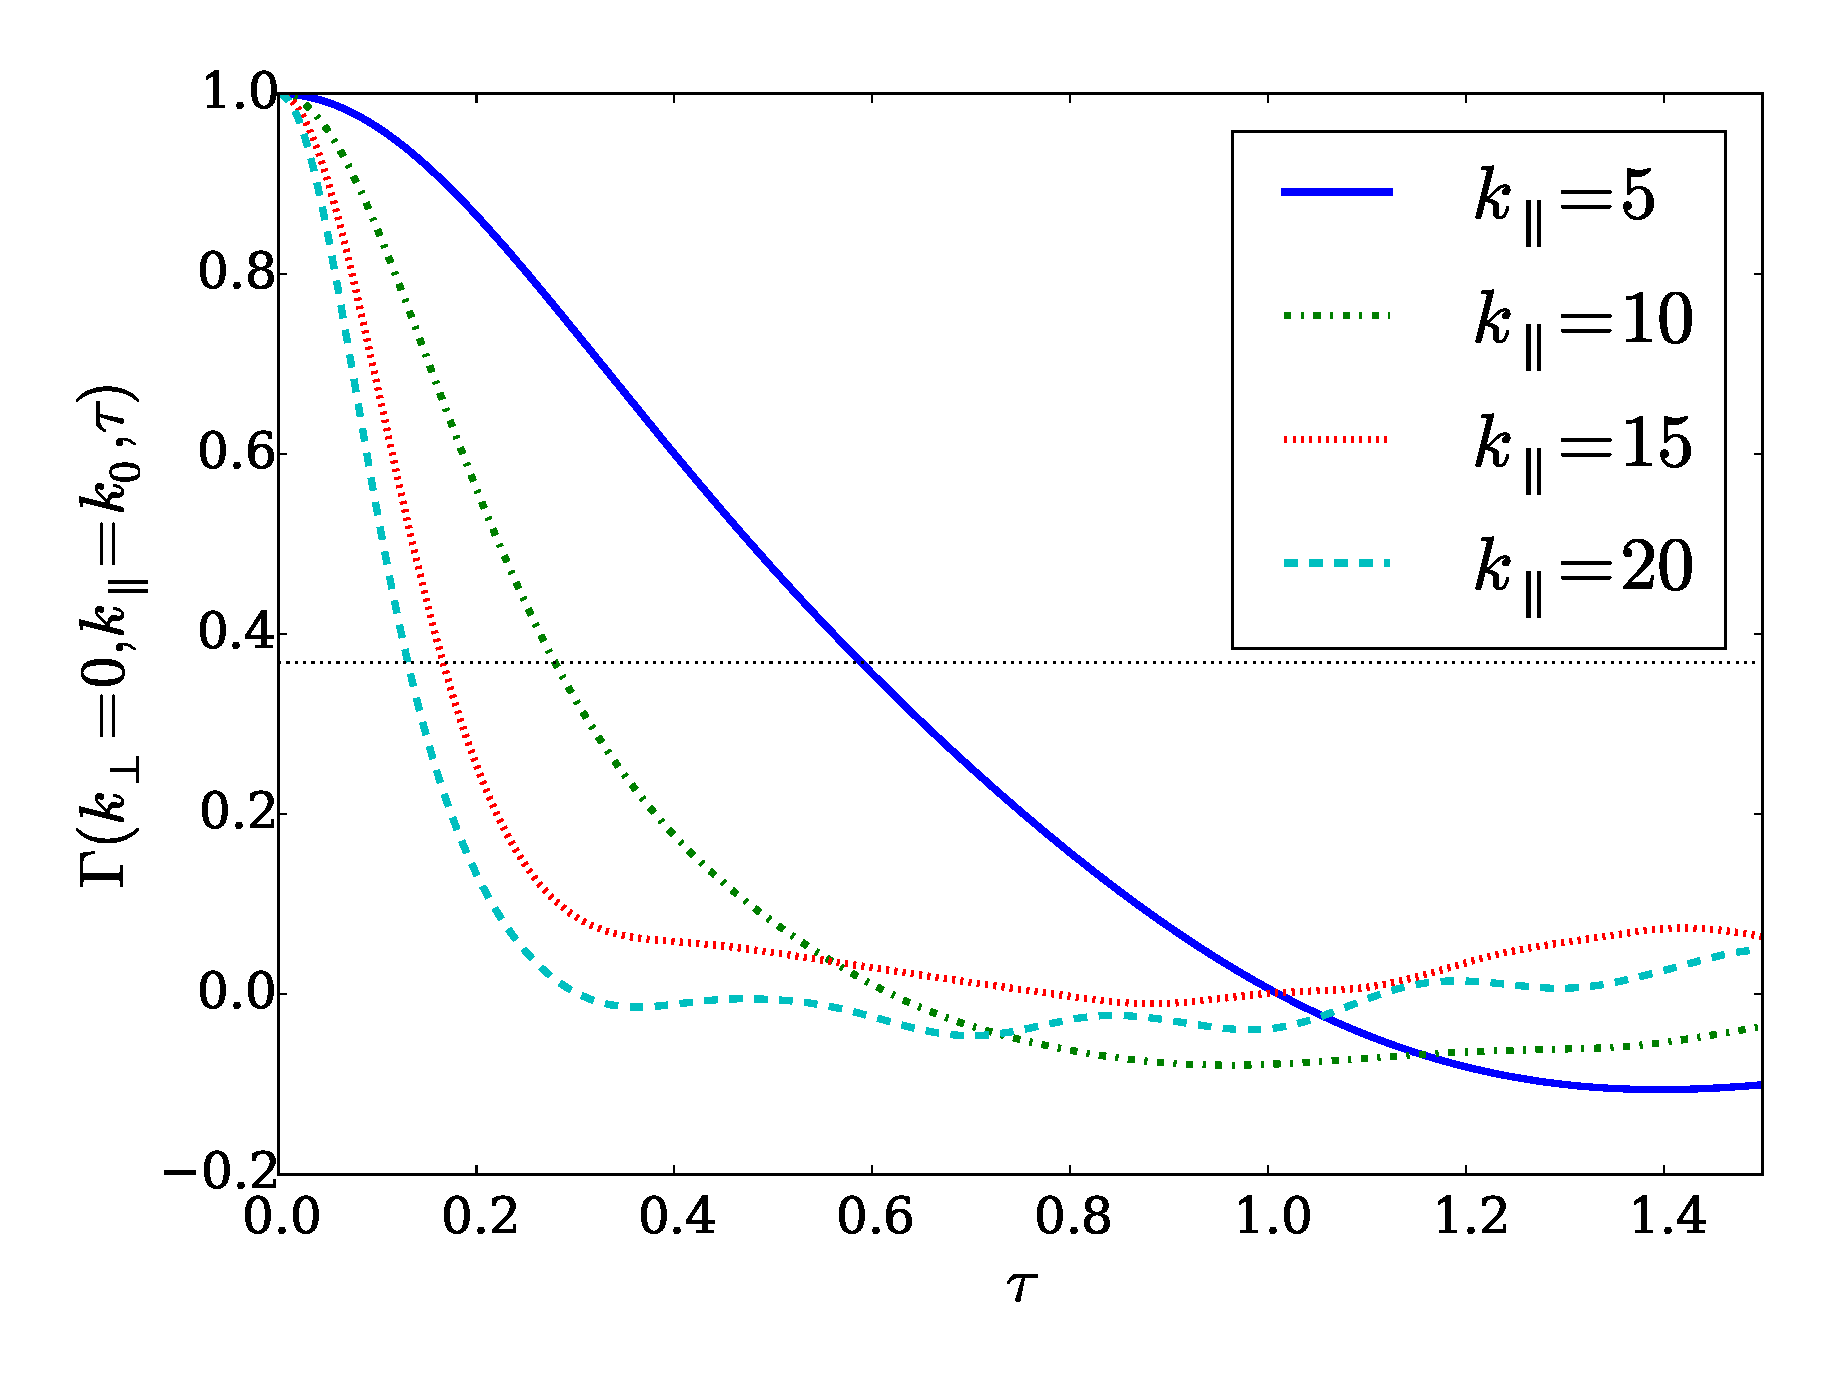
\includegraphics[width=0.9\columnwidth]{P1/fig4_B1_b_kperp.eps}
      \end{center}
    \end{minipage}
    \column{0.5\textwidth}
    \begin{minipage}[t]{1\textwidth}
      \begin{center}
        $\Gamma(k_\perp=k_0,k_\parallel=0,\tau)$ \\
        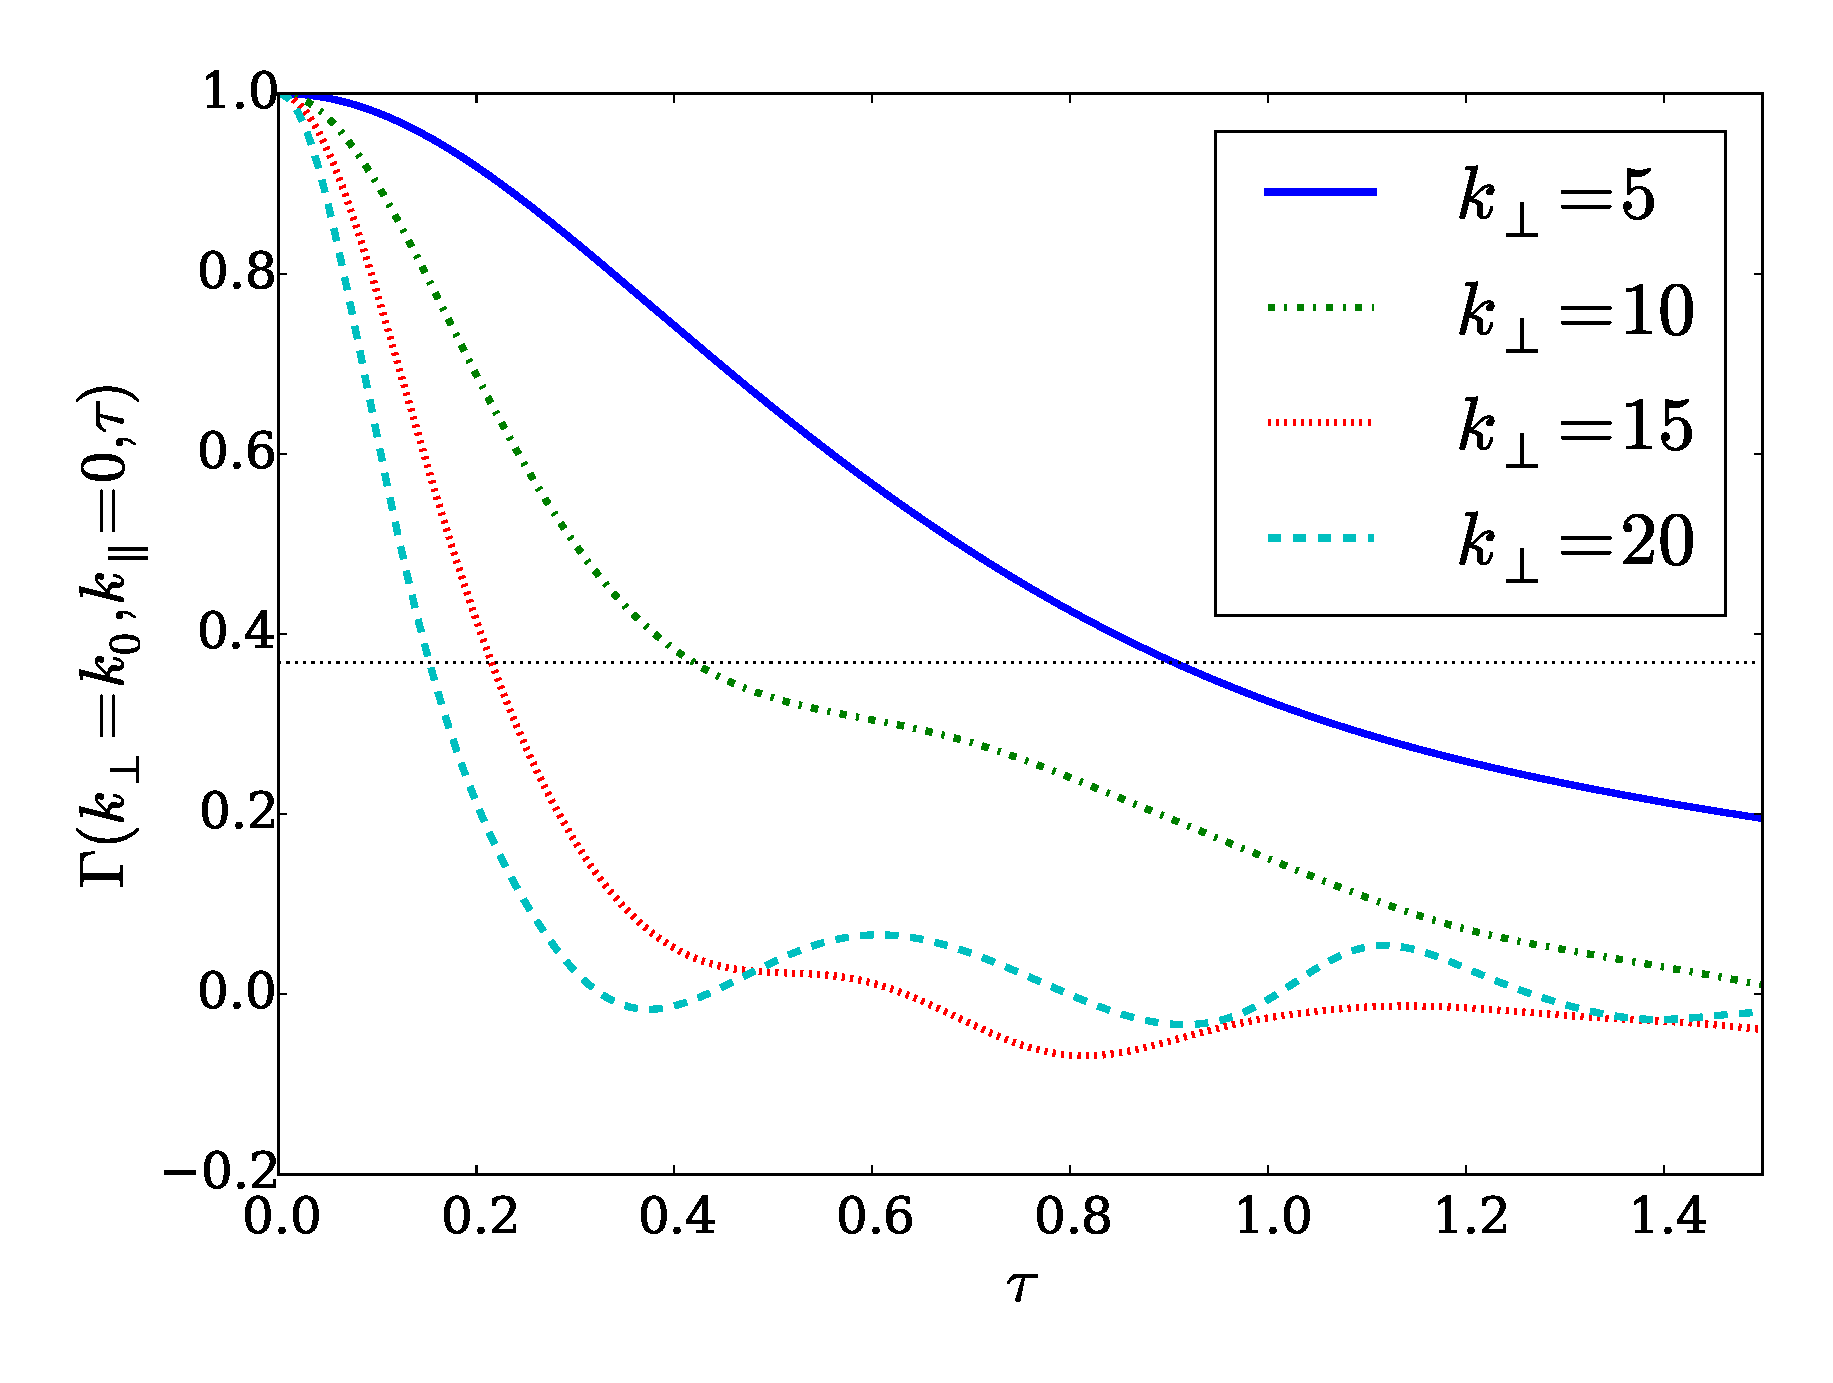
\includegraphics[width=0.9\columnwidth]{P1/fig4_B1_b_kpara.eps}
      \end{center}
    \end{minipage}
  \end{columns}
}
\note[itemize]{
\item ¿Qué tiempo controla la descorrelación temporal? Mecesitamos comparar el
  tiempo de descorrelación en las distintas escalas con el
  comportamiento teórico esperado para cada proceso físico.
\item Correlación aproximadamente decaimiento exponencial
  $\Gamma(\vec{k},\tau) \sim e^{-\tau/\tau_D(\vec{k})}$
\item El valor de $\tau$ para el cual $\Gamma=1/e$ corresponde al
  tiempo de descorrelación $\tau_D$ para cada valor de $\vec{k}$.
}

  


\frame{\frametitle{Tiempos de descorrelación}
  \pause
  {\Large \underline{Tiempo de descorrelación para el caso isotrópico $B_0=0$}}
  \begin{center}
    \includegraphics[width=0.7\columnwidth]{P1/fig5_B0_b.eps}
  \end{center}
}
\note[itemize]{
\item $\tau_D$ se encuentra en buen acuerdo con $\tau_{sw}$.
\item Resultados consistentes con Servidio (2011).
}


\frame{\frametitle{Tiempos de descorrelación}
  {\Large \underline{Tiempos de descorrelación: $B_0=1$ y $k_\perp = k_0$}}
  \begin{columns}
    \column{0.5\textwidth}
    \begin{minipage}[t]{1\textwidth}
      \begin{center}
        $k_\perp = 0$\\
        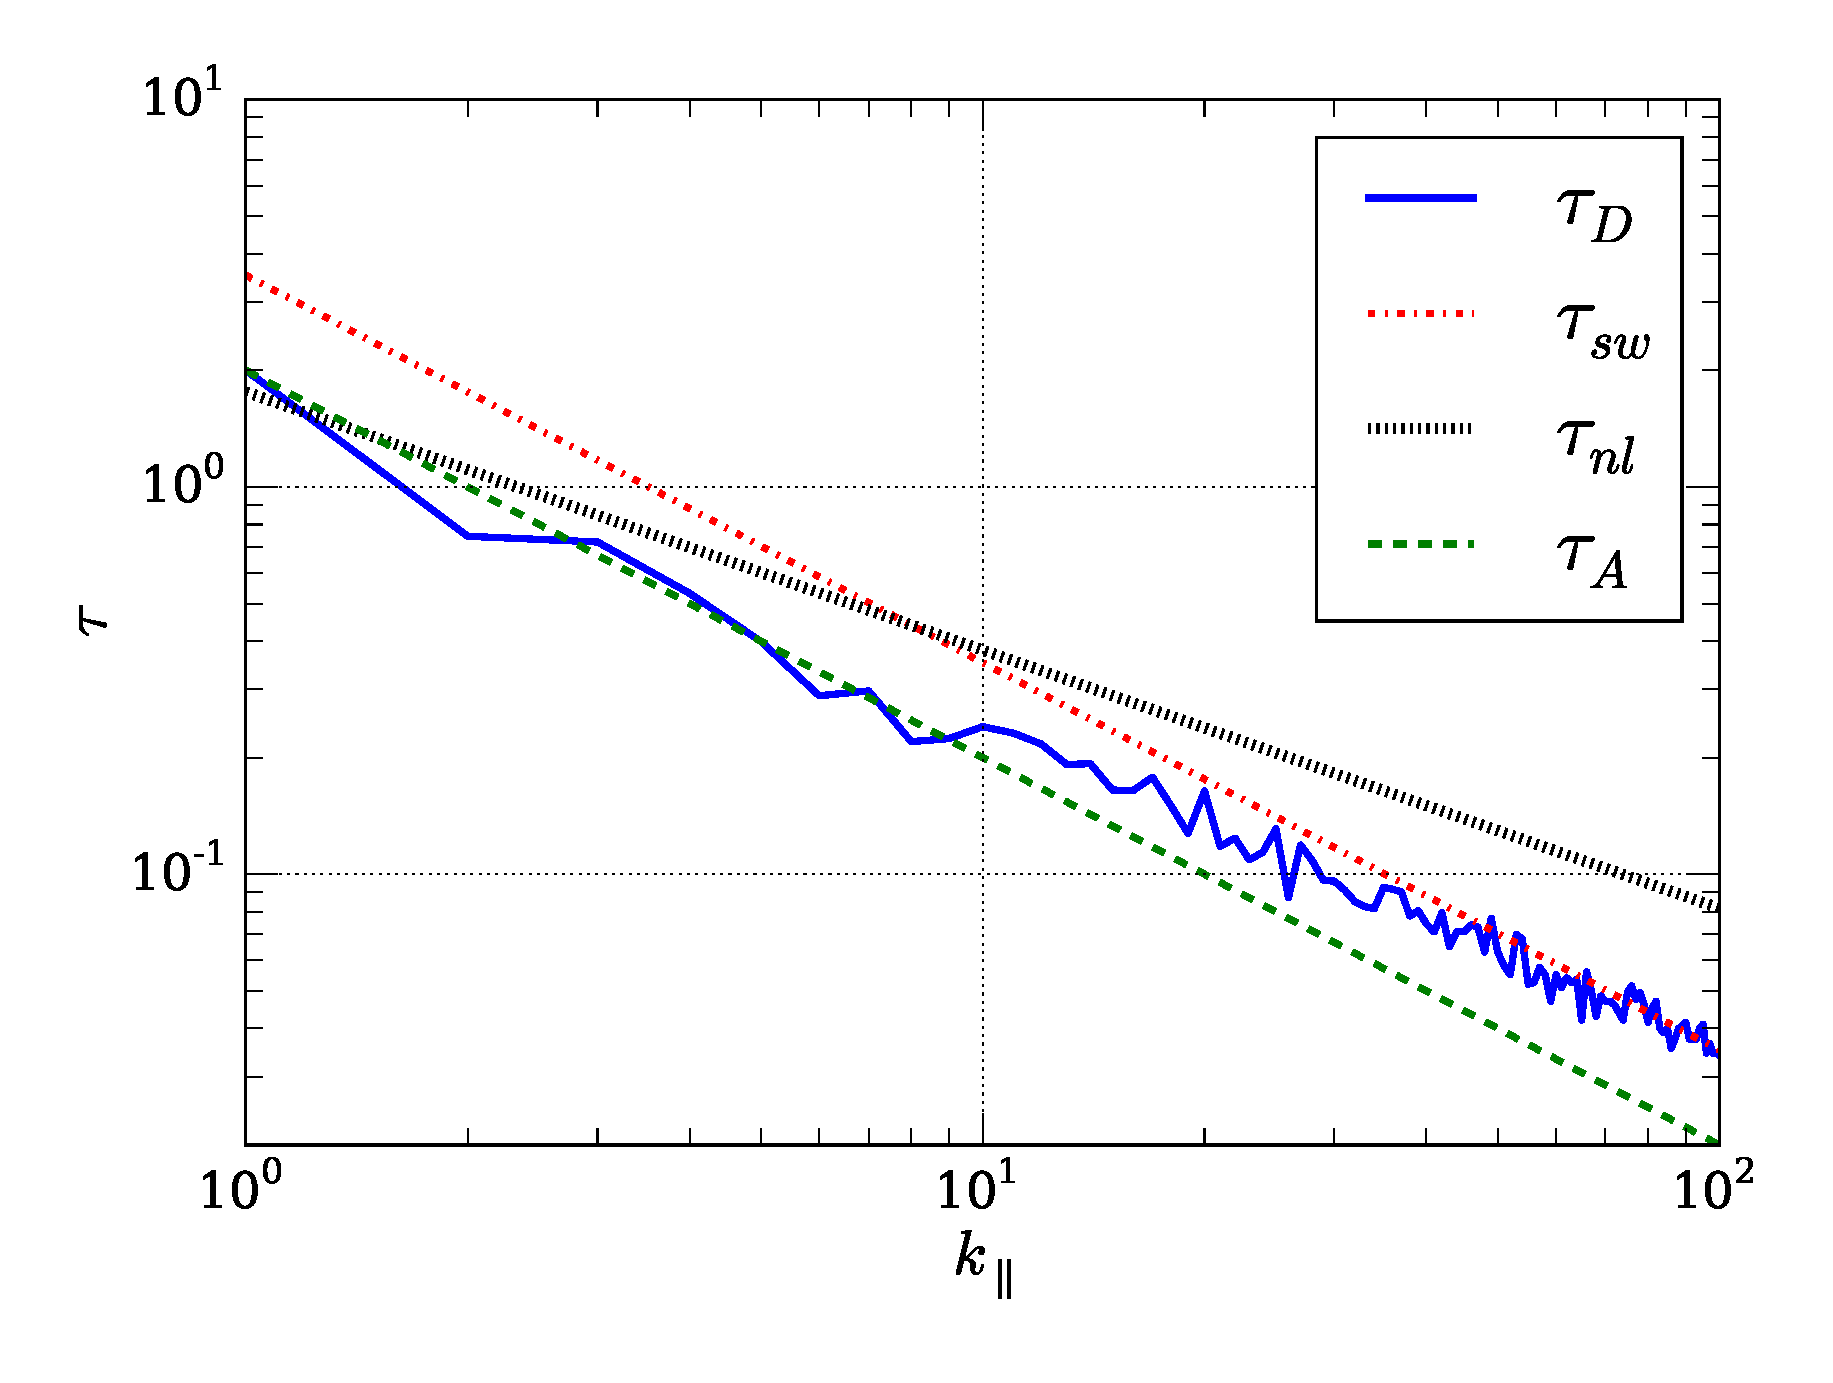
\includegraphics[width=0.76\columnwidth]{P1/fig5_B1_b_kperp_0.eps}
      \end{center}
    \end{minipage}
    \column{0.5\textwidth}
    \begin{minipage}[t]{1\textwidth}
      \begin{center}
        $k_\perp = 10$\\
        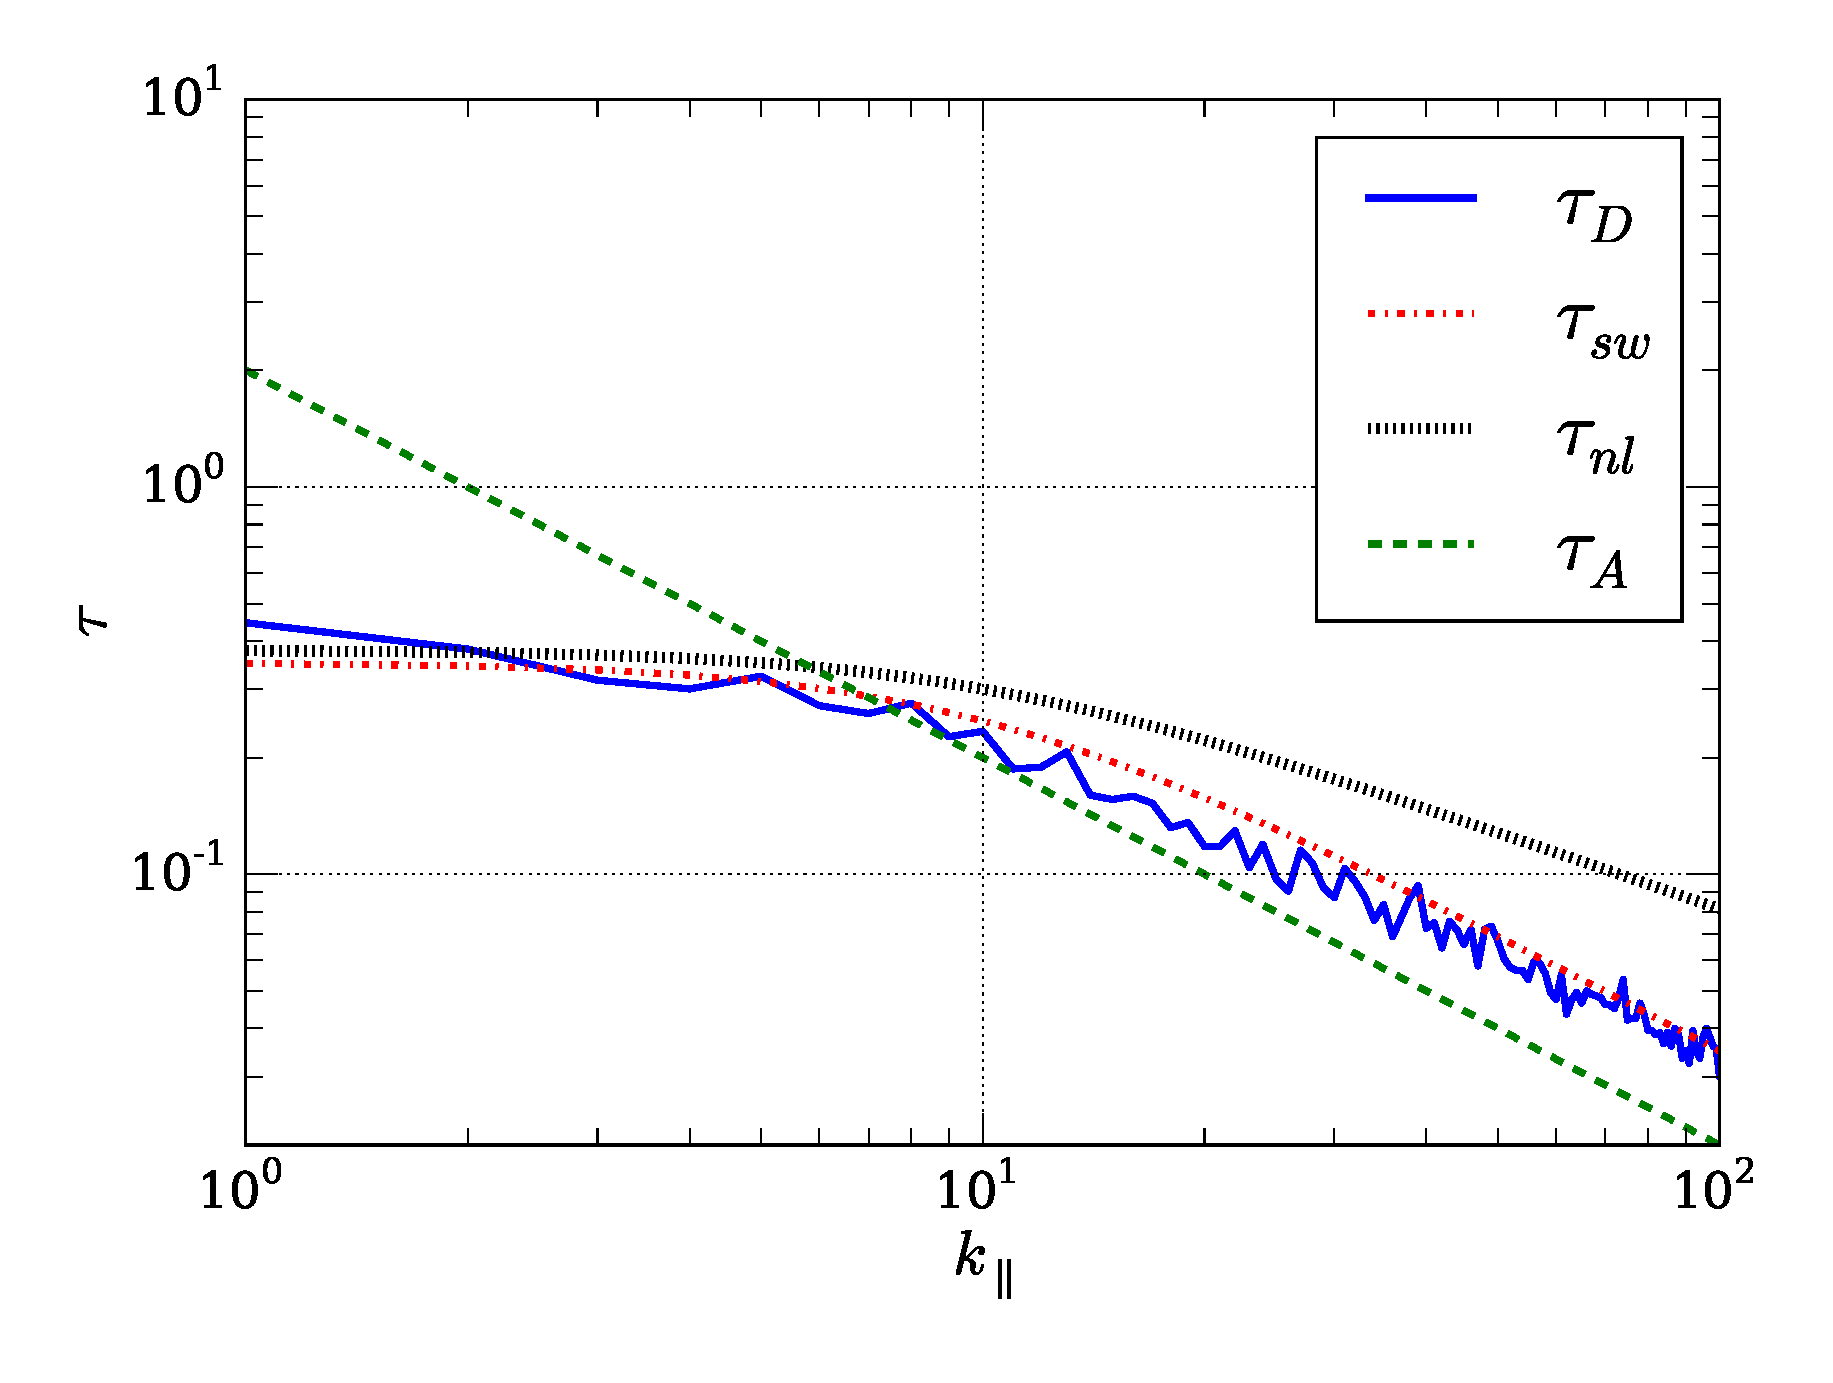
\includegraphics[width=0.76\columnwidth]{P1/fig5_B1_b_kperp_10.eps}
      \end{center}
    \end{minipage}
  \end{columns}
  \vspace{-0.5cm}
  \begin{center}
    $k_\perp = 20$\\
    \includegraphics[width=0.38\columnwidth]{P1/fig5_B1_b_kperp_20.eps} \\
  \end{center}
}
\note[itemize]{
\item En el caso general, \textit{sweeping} y Alfvén escalan como
  $k^{-1}$. Con campo guía, podemos usar que Alfvén sólo escala con
  $k_\parallel$.
\item \emph{sweeping} domina $k$ grande, y Alfvén $k$ chico.
}



\frame{\frametitle{Tiempos de descorrelación}
  {\Large \underline{Tiempos de descorrelación: $B_0=1$ y $k_\parallel = k_0$}}
  \begin{columns}
    \column{0.5\textwidth}
    \begin{minipage}[t]{1\textwidth}
      \begin{center}
        $k_\parallel = 0$\\
        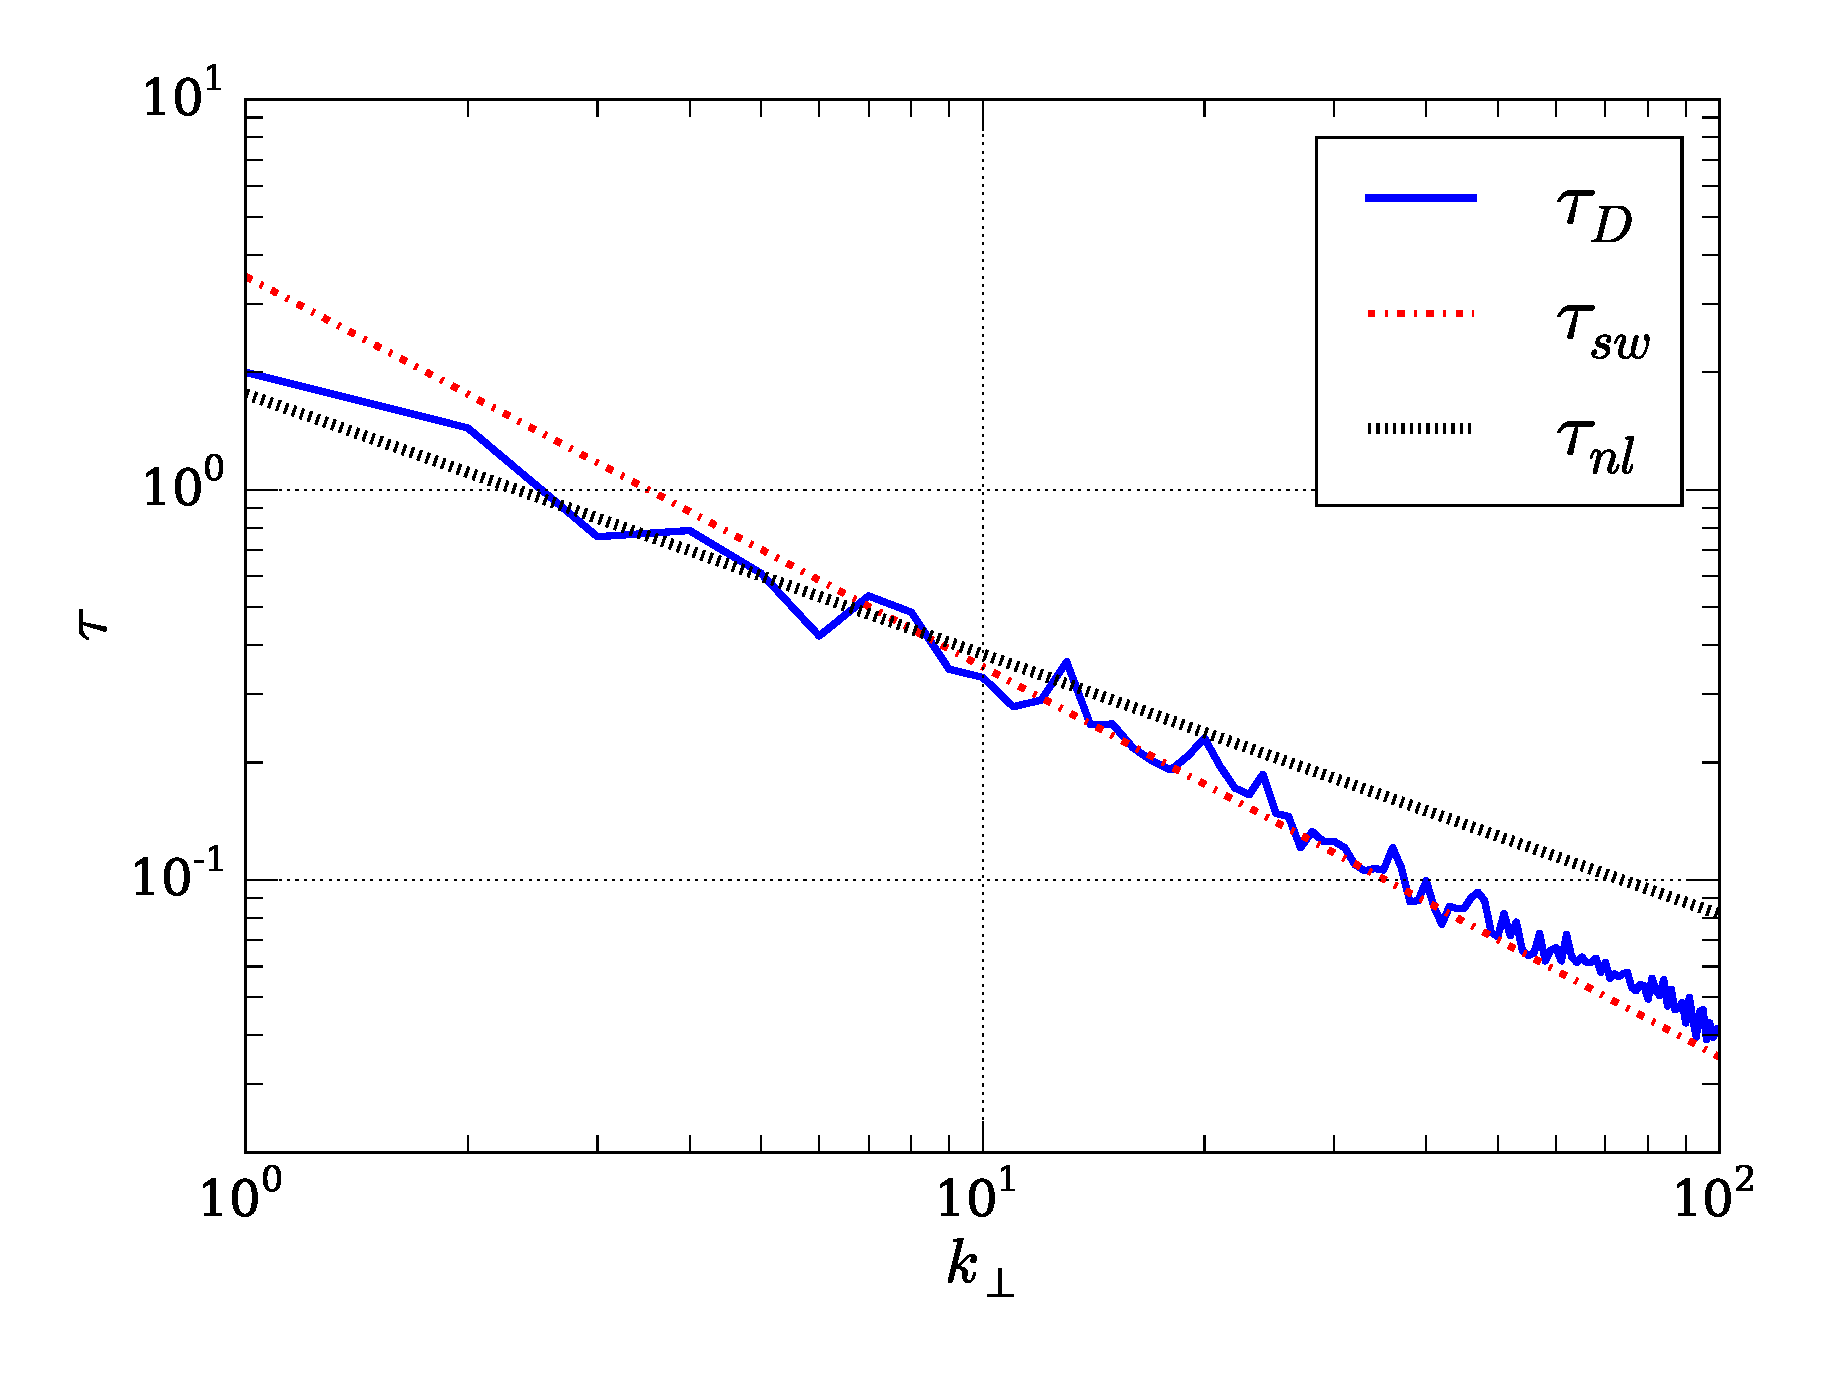
\includegraphics[width=0.76\columnwidth]{P1/fig5_B1_b_kpara_0.eps}
      \end{center}
    \end{minipage}
    \column{0.5\textwidth}
    \begin{minipage}[t]{1\textwidth}
      \begin{center}
        $k_\parallel = 10$\\
        \includegraphics[width=0.76\columnwidth]{P1/fig5_B1_b_kpara_10.eps}
      \end{center}
    \end{minipage}
  \end{columns}
  \vspace{-0.5cm}
  \begin{center}
    $k_\parallel = 20$\\
    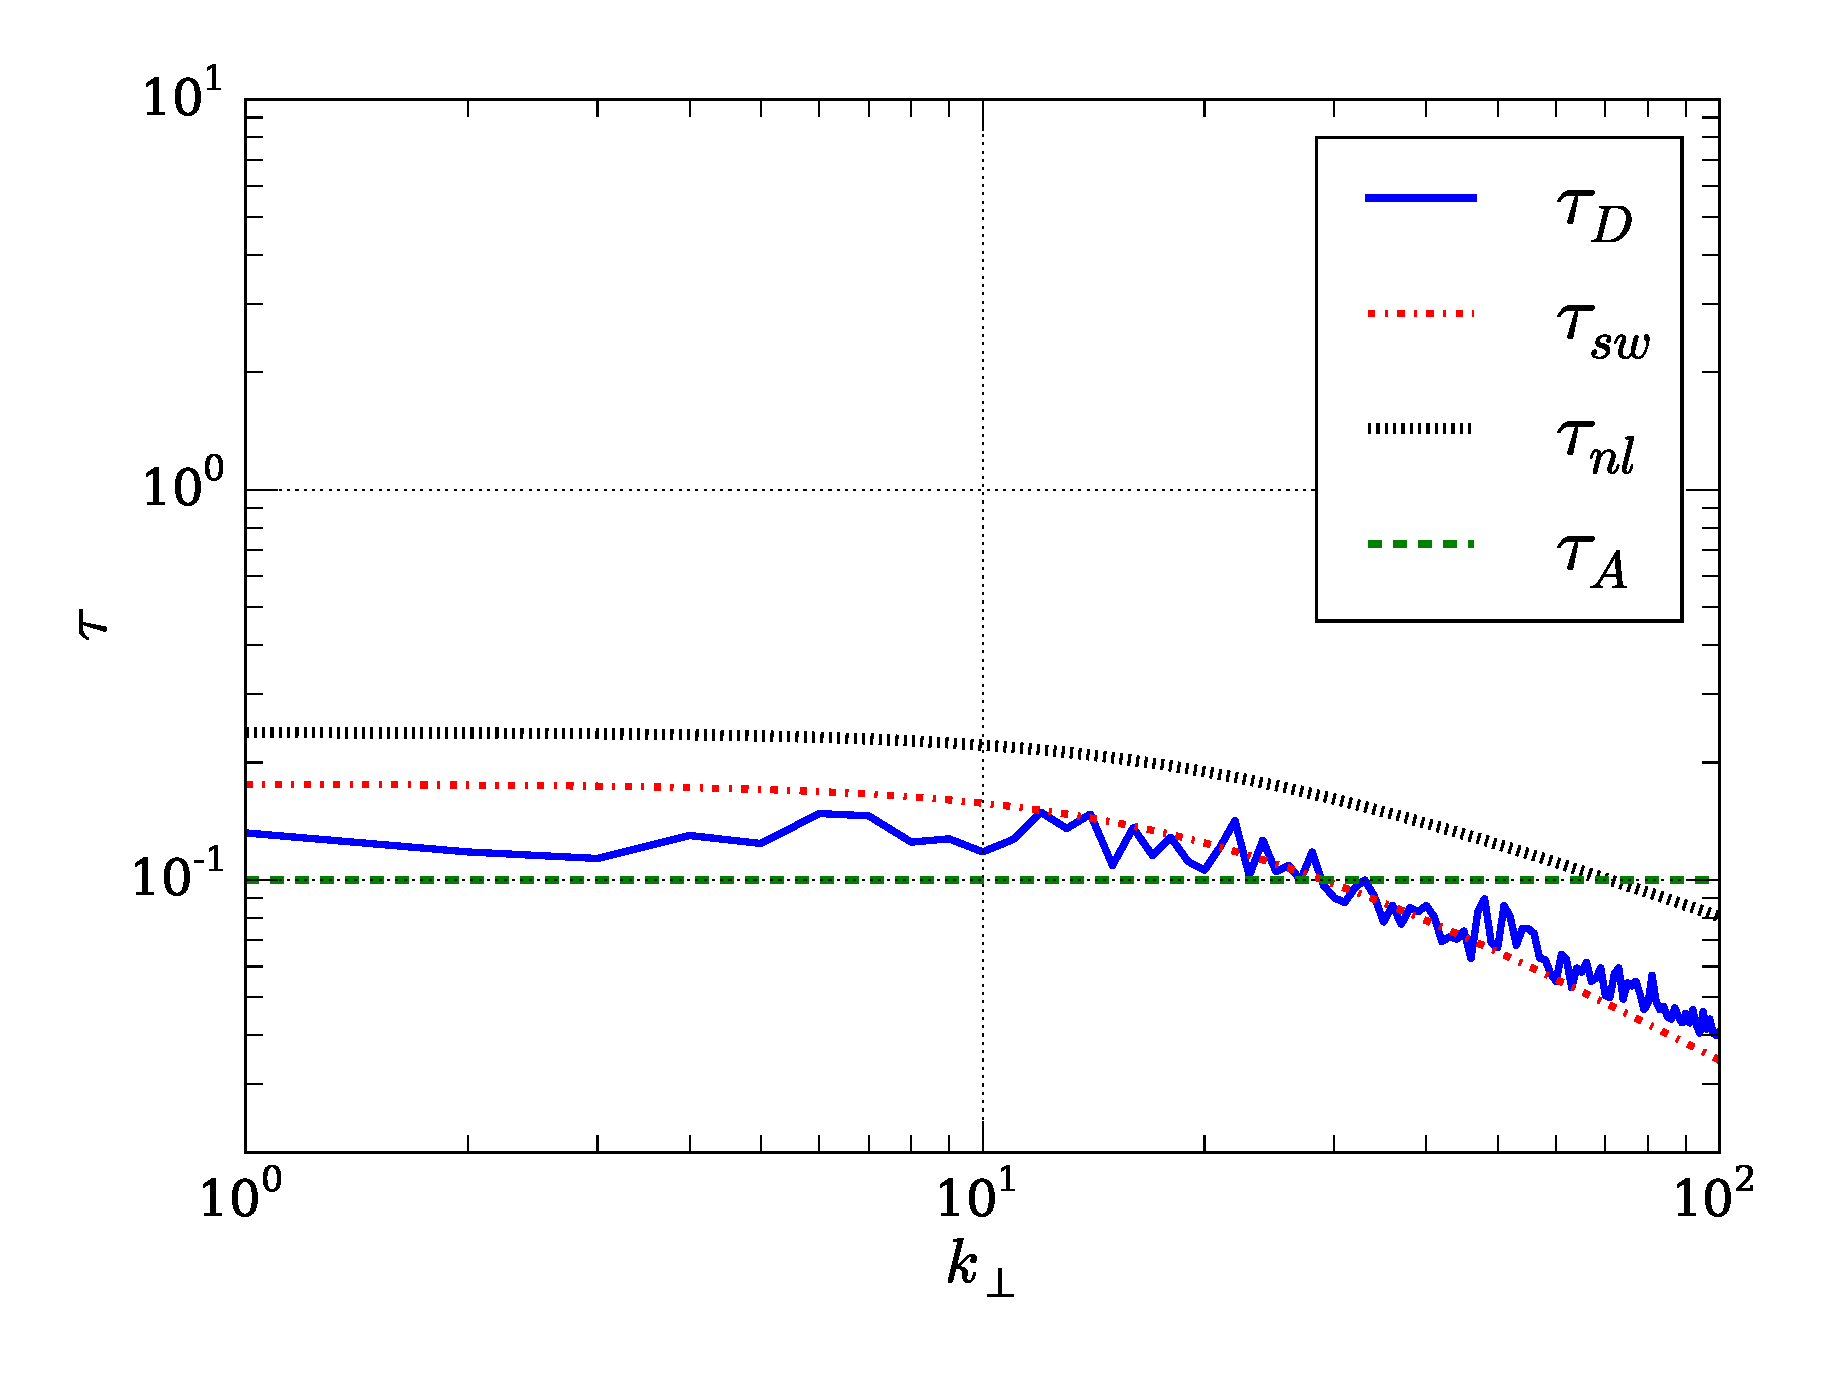
\includegraphics[width=0.38\columnwidth]{P1/fig5_B1_b_kpara_20.eps} \\
  \end{center}
}


\frame{\frametitle{Tiempos de descorrelación}
  {\Large \underline{Tiempos de descorrelación: $B_0=0.25$ y $k_\perp = k_0$}}
  \begin{columns}
    \column{0.5\textwidth}
    \begin{minipage}[t]{1\textwidth}
      \begin{center}
        $k_\perp = 0$\\
        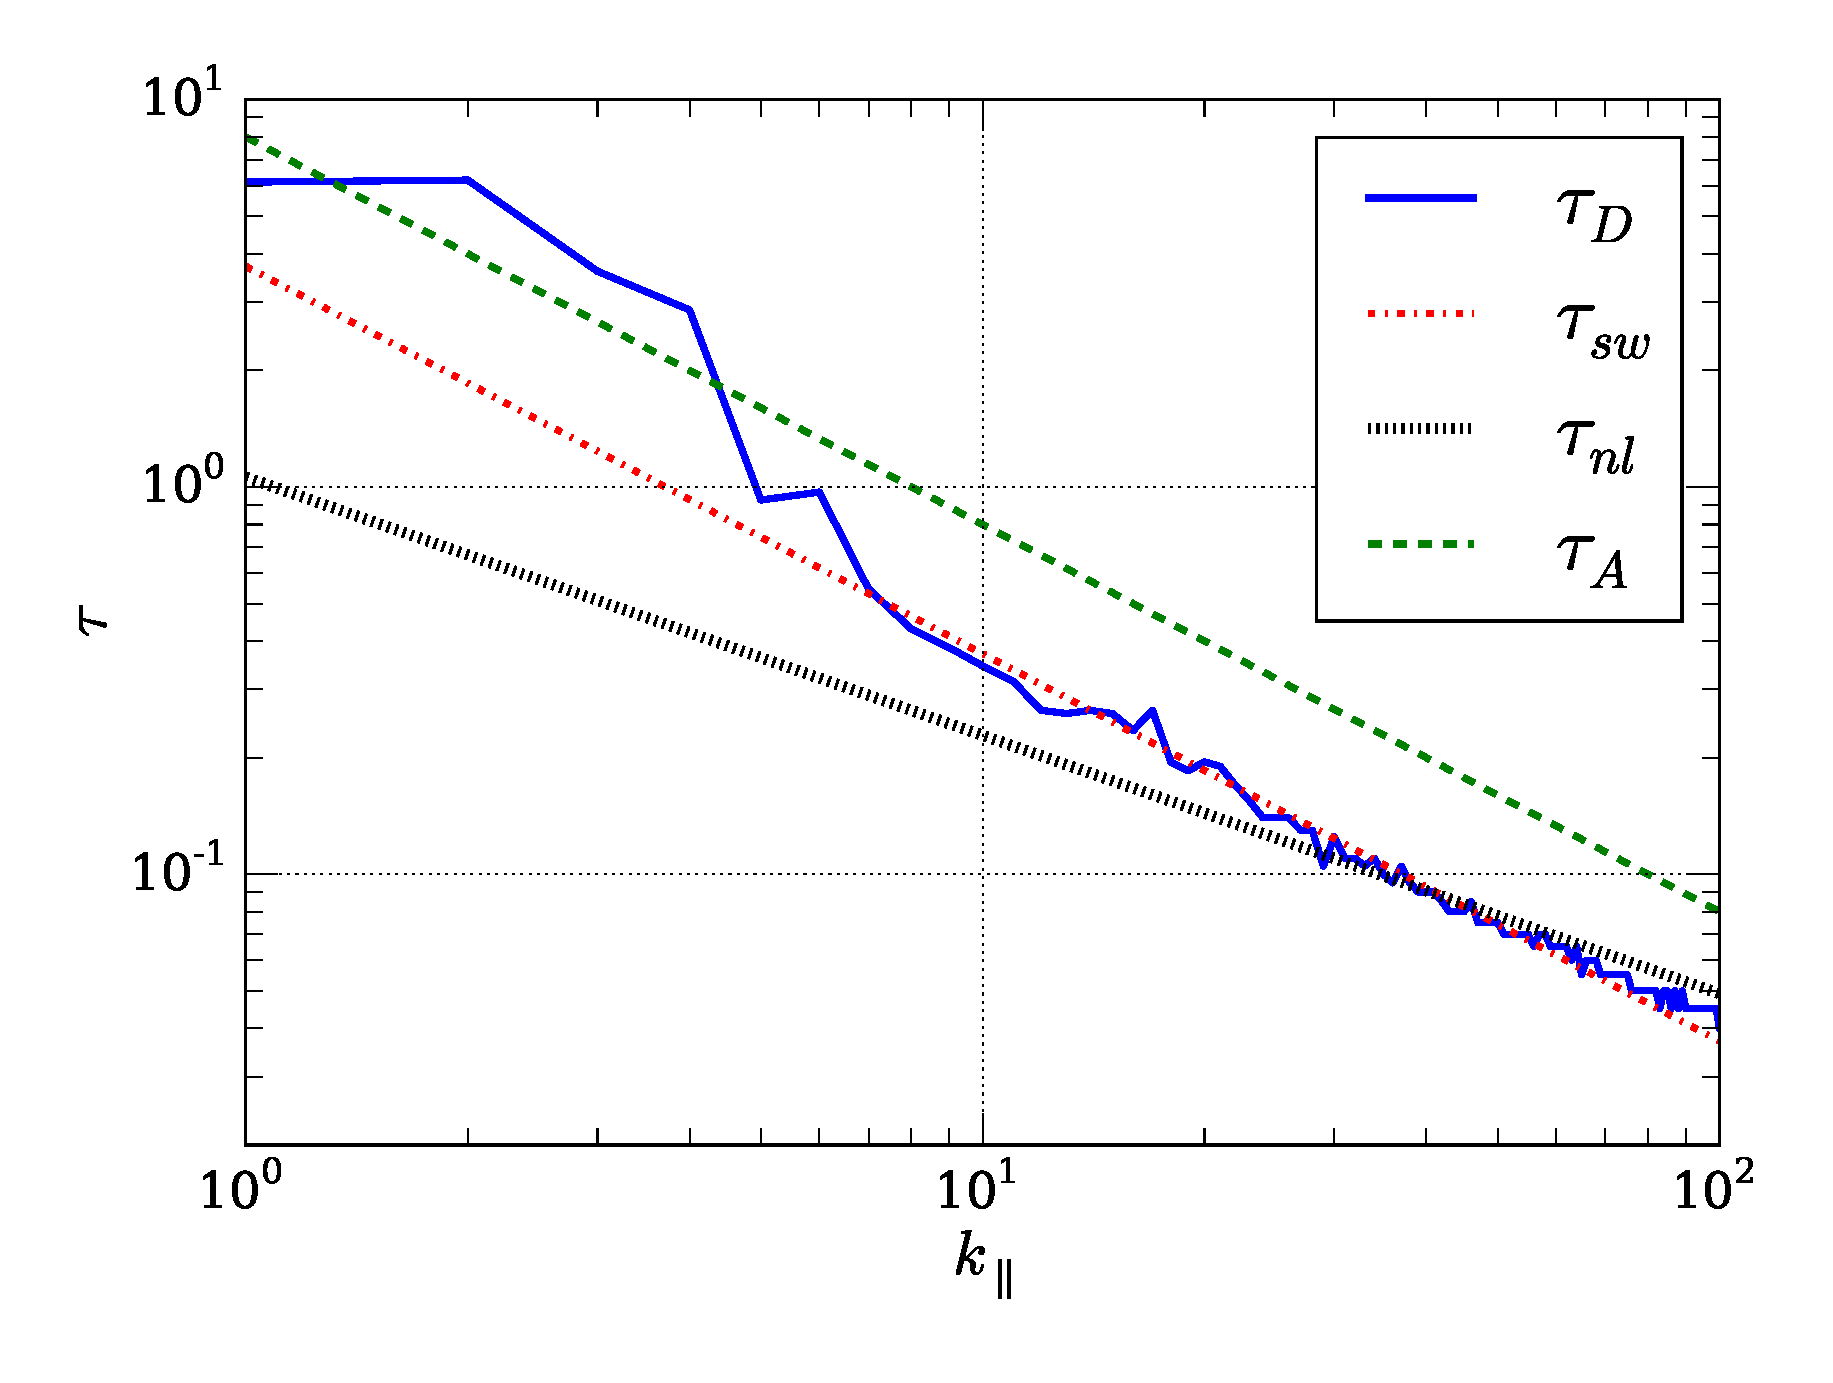
\includegraphics[width=0.76\columnwidth]{P1/fig5_B025_b_kperp_0.eps}
      \end{center}
    \end{minipage}
    \column{0.5\textwidth}
    \begin{minipage}[t]{1\textwidth}
      \begin{center}
        $k_\perp = 10$\\
        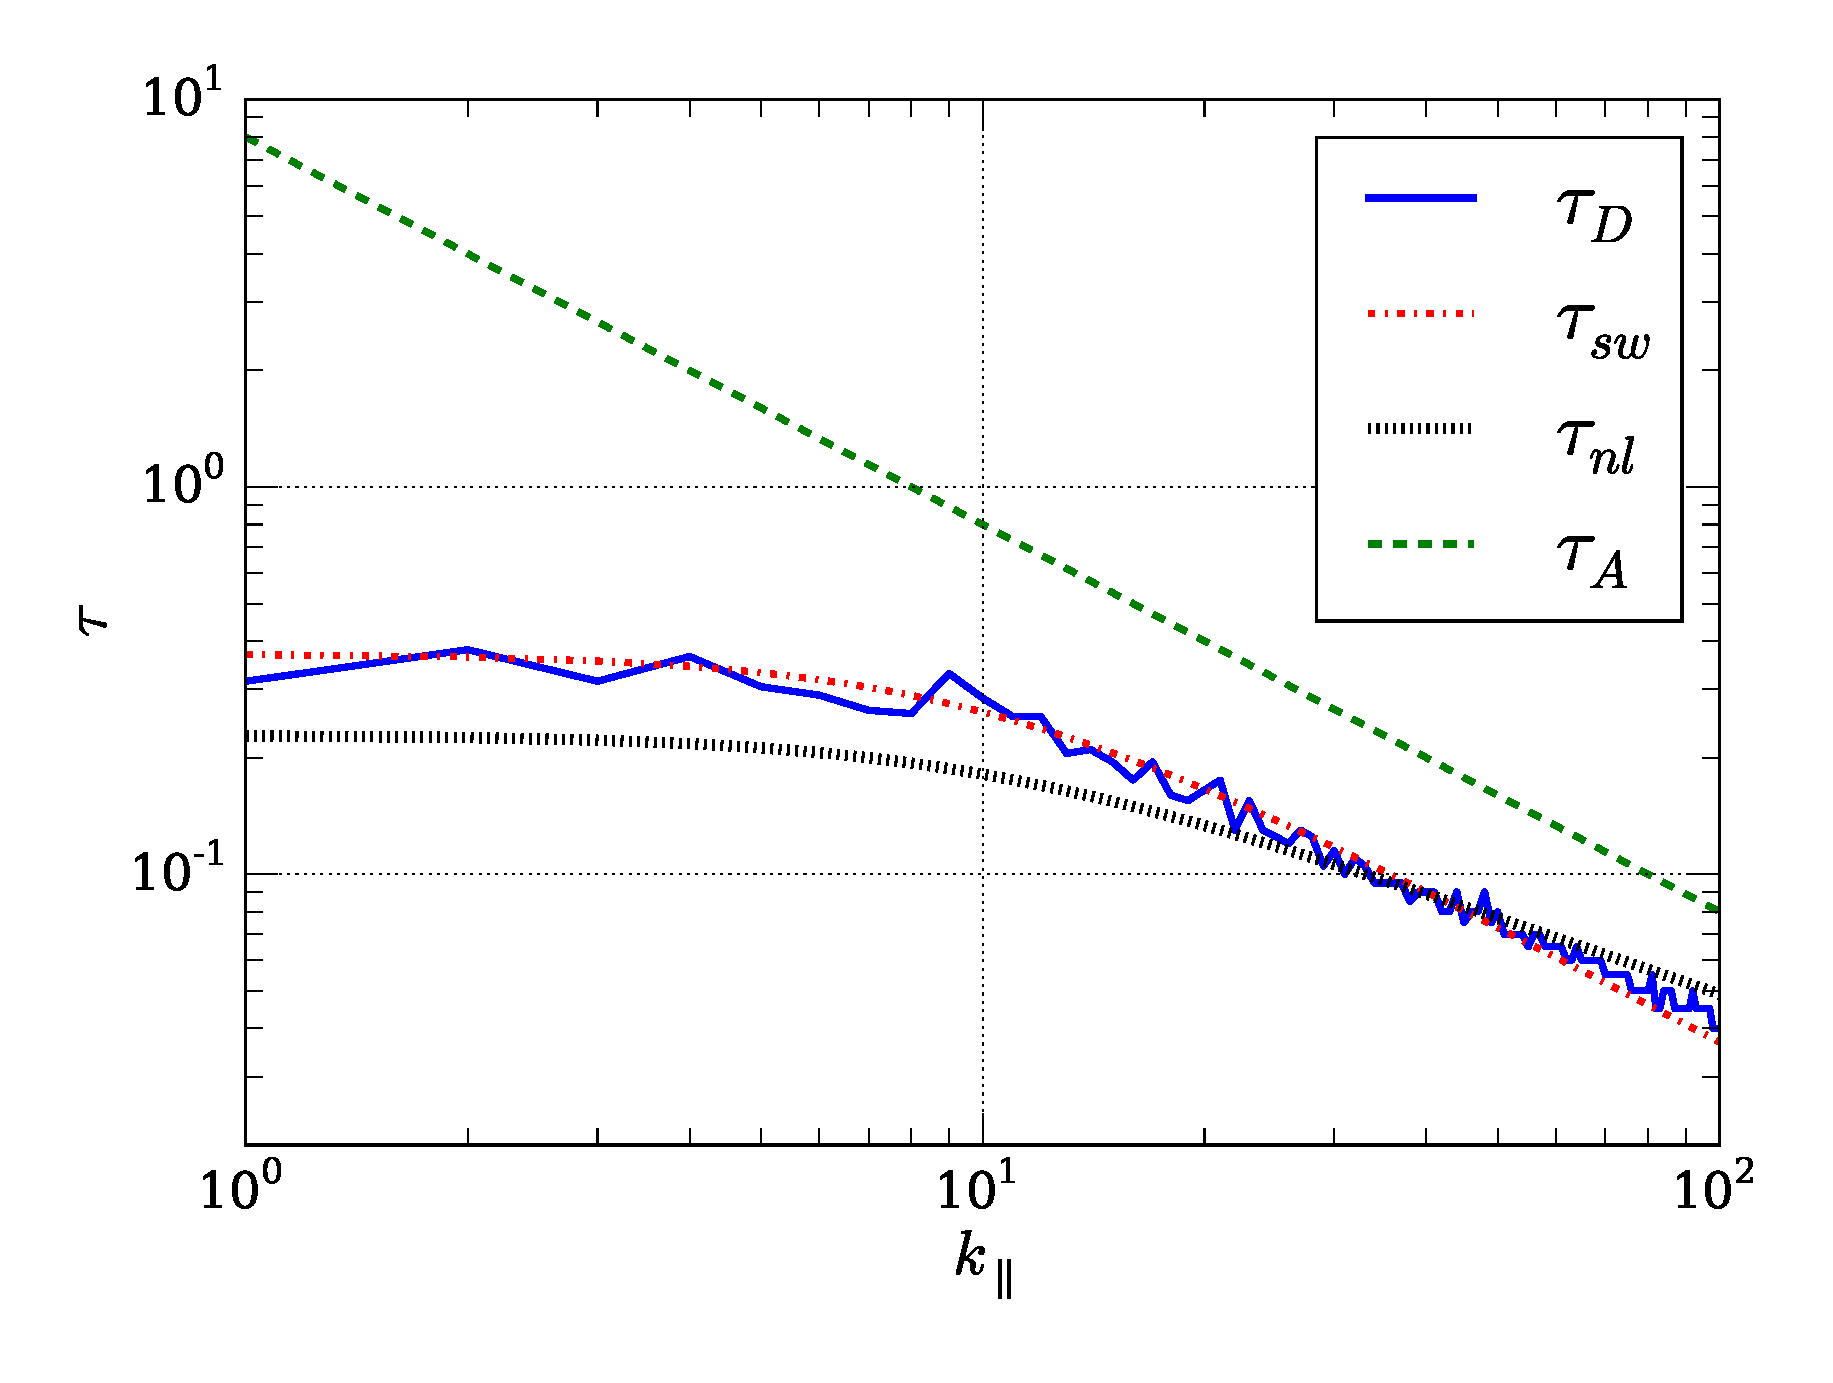
\includegraphics[width=0.76\columnwidth]{P1/fig5_B025_b_kperp_10.eps}
      \end{center}
    \end{minipage}
  \end{columns}
  \vspace{-0.5cm}
  \begin{center}
    $k_\perp = 20$\\
    \includegraphics[width=0.38\columnwidth]{P1/fig5_B025_b_kperp_20.eps} \\
  \end{center}
}
\note[itemize]{
\item Tiempos de descorrelación más cercanos al tiempo de
  \textit{sweeping}. Consistente con el resultado del espectro
  energético.
}


\frame{\frametitle{Tiempos de descorrelación}
  {\Large \underline{Tiempos de descorrelación: $B_0=0.25$ y $k_\parallel = k_0$}}
  \begin{columns}
    \column{0.5\textwidth}
    \begin{minipage}[t]{1\textwidth}
      \begin{center}
        $k_\parallel = 0$\\
        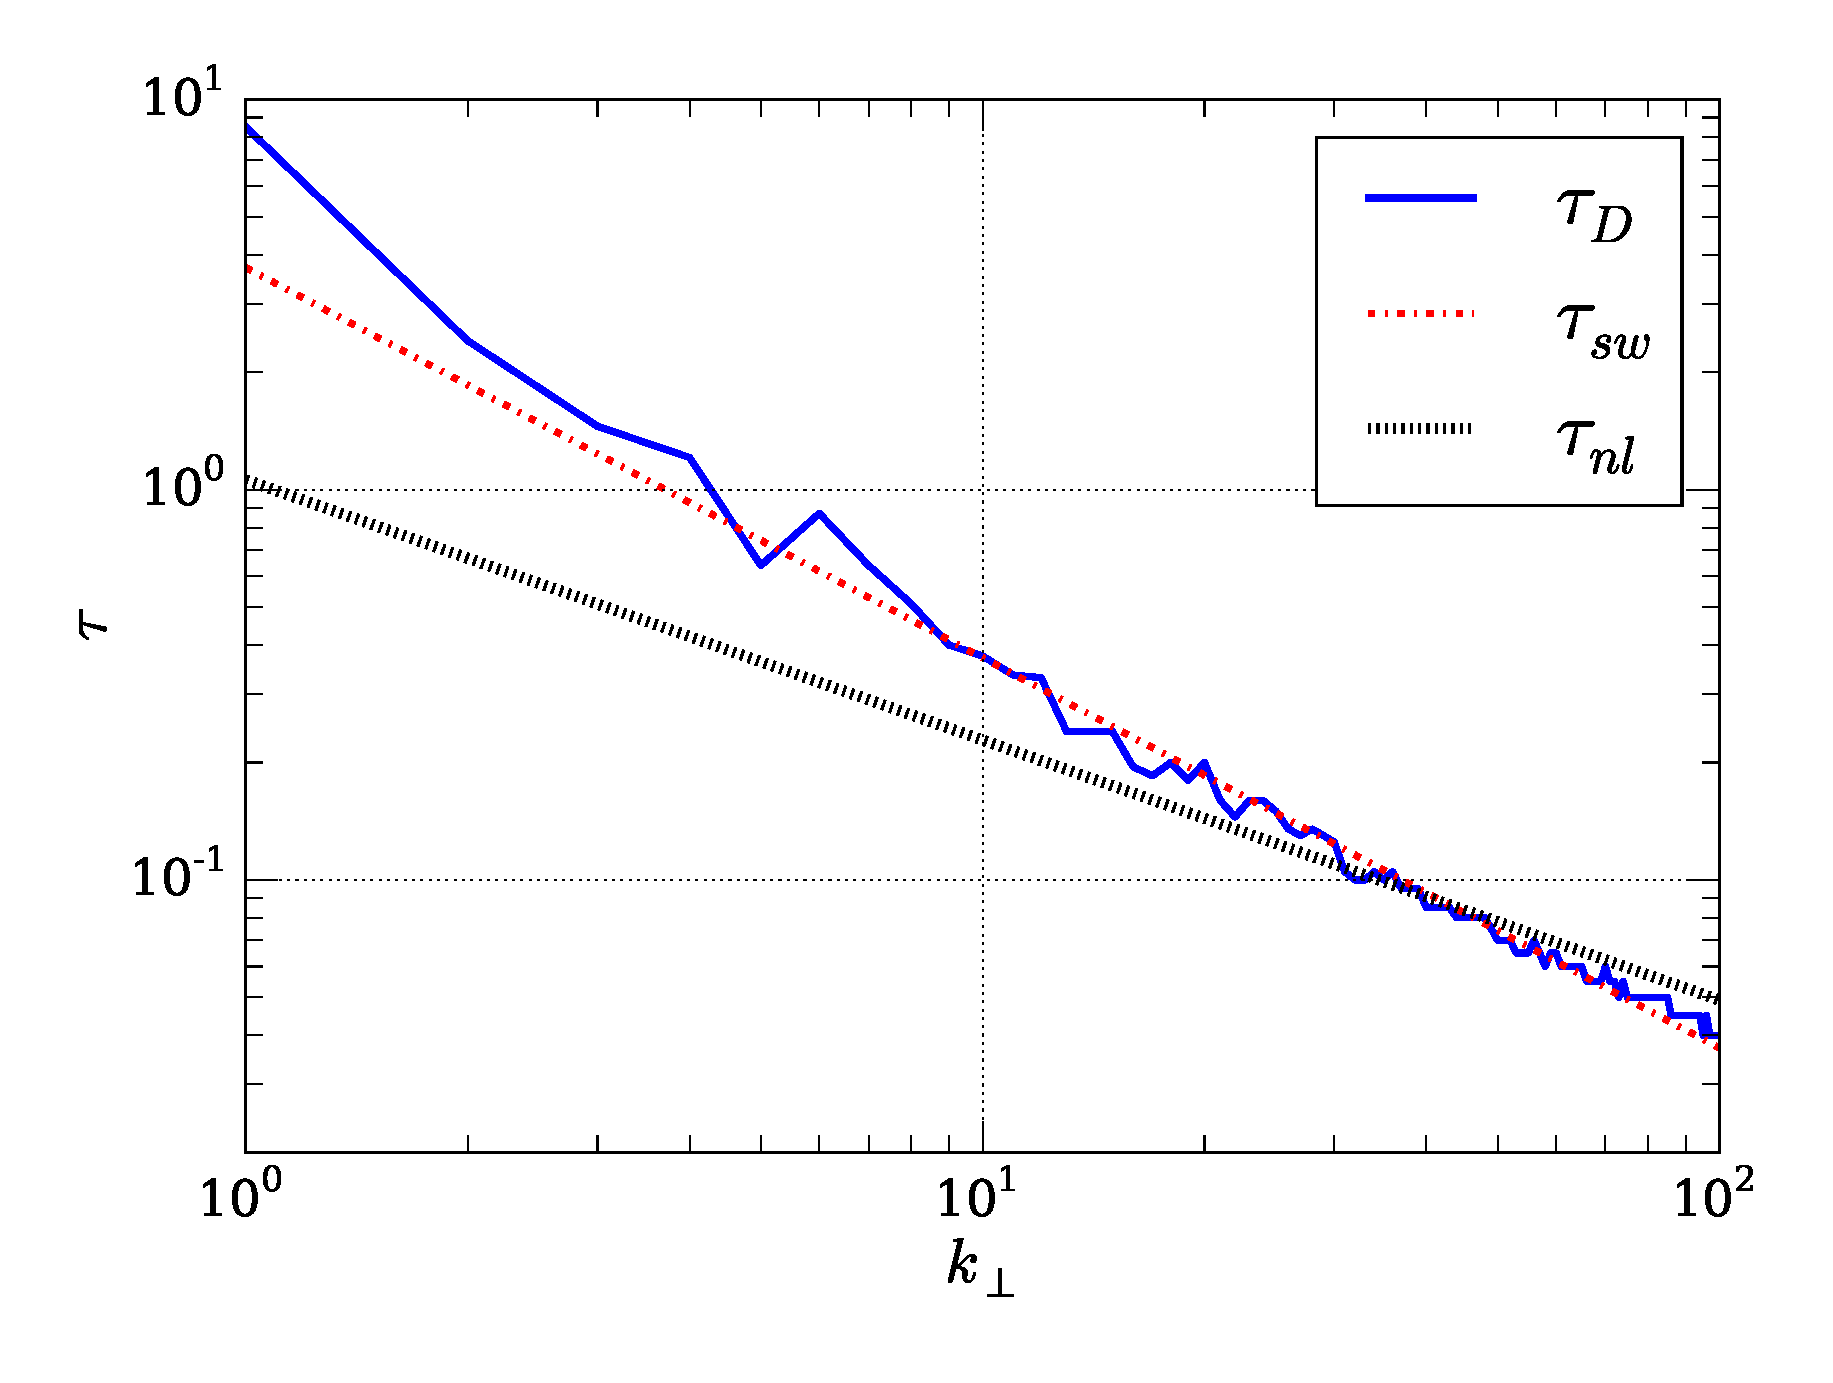
\includegraphics[width=0.76\columnwidth]{P1/fig5_B025_b_kpara_0.eps}
      \end{center}
    \end{minipage}
    \column{0.5\textwidth}
    \begin{minipage}[t]{1\textwidth}
      \begin{center}
        $k_\parallel = 10$\\
        \includegraphics[width=0.76\columnwidth]{P1/fig5_B025_b_kpara_10.eps}
      \end{center}
    \end{minipage}
  \end{columns}
  \vspace{-0.5cm}
  \begin{center}
    $k_\parallel = 20$\\
    \includegraphics[width=0.38\columnwidth]{P1/fig5_B025_b_kpara_20.eps} \\
  \end{center}
}
\note[itemize]{
\item 
}


\frame{\frametitle{Tiempos de descorrelación}
  {\Large \underline{Tiempos de descorrelación: $B_0=8$ y $k_\perp = k_0$}}
  \begin{columns}
    \column{0.5\textwidth}
    \begin{minipage}[t]{1\textwidth}
      \begin{center}
        $k_\perp = 0$\\
        \includegraphics[width=0.76\columnwidth]{P1/fig5_B8_b_kperp_0.eps}
      \end{center}
    \end{minipage}
    \column{0.5\textwidth}
    \begin{minipage}[t]{1\textwidth}
      \begin{center}
        $k_\perp = 10$\\
        \includegraphics[width=0.76\columnwidth]{P1/fig5_B8_b_kperp_10.eps}
      \end{center}
    \end{minipage}
  \end{columns}
  \vspace{-0.5cm}
  \begin{center}
    $k_\perp = 20$\\
    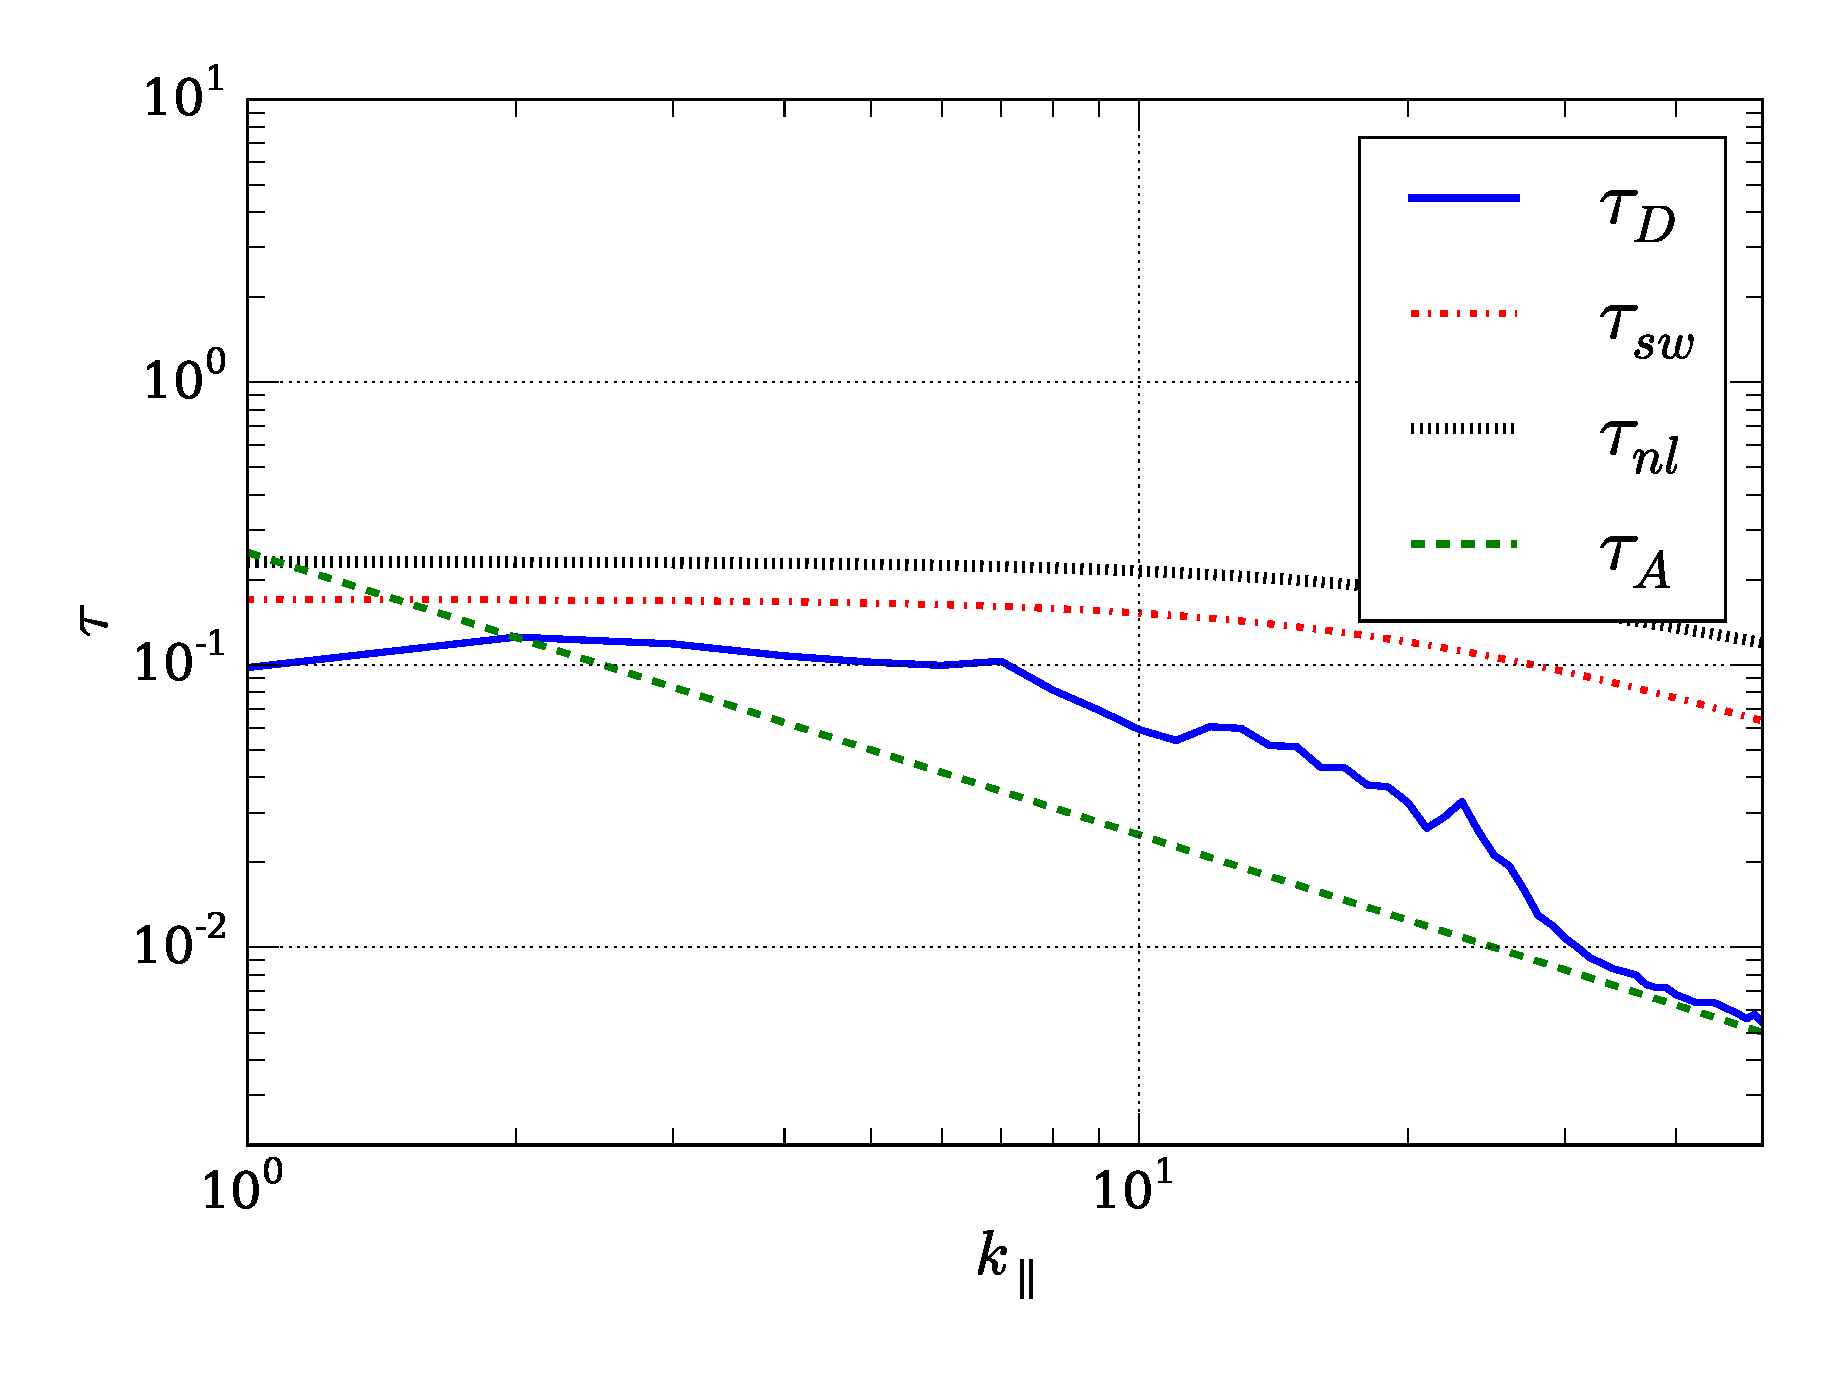
\includegraphics[width=0.38\columnwidth]{P1/fig5_B8_b_kperp_20.eps} \\
  \end{center}
}
\note[itemize]{
\item Para valores pequeños de $k_\perp$, el tiempo de Alfvén
  domina. Después, $\tau_D$ se acerca al \emph{sweeping}.
}




\frame{\frametitle{Tiempos de descorrelación}
  {\Large \underline{Tiempos de descorrelación: $B_0=8$ y $k_\parallel = k_0$}}
  \begin{columns}
    \column{0.5\textwidth}
    \begin{minipage}[t]{1\textwidth}
      \begin{center}
        $k_\parallel = 0$\\
        \includegraphics[width=0.76\columnwidth]{P1/fig5_B8_b_kpara_0.eps}
      \end{center}
    \end{minipage}
    \column{0.5\textwidth}
    \begin{minipage}[t]{1\textwidth}
      \begin{center}
        $k_\parallel = 10$\\
        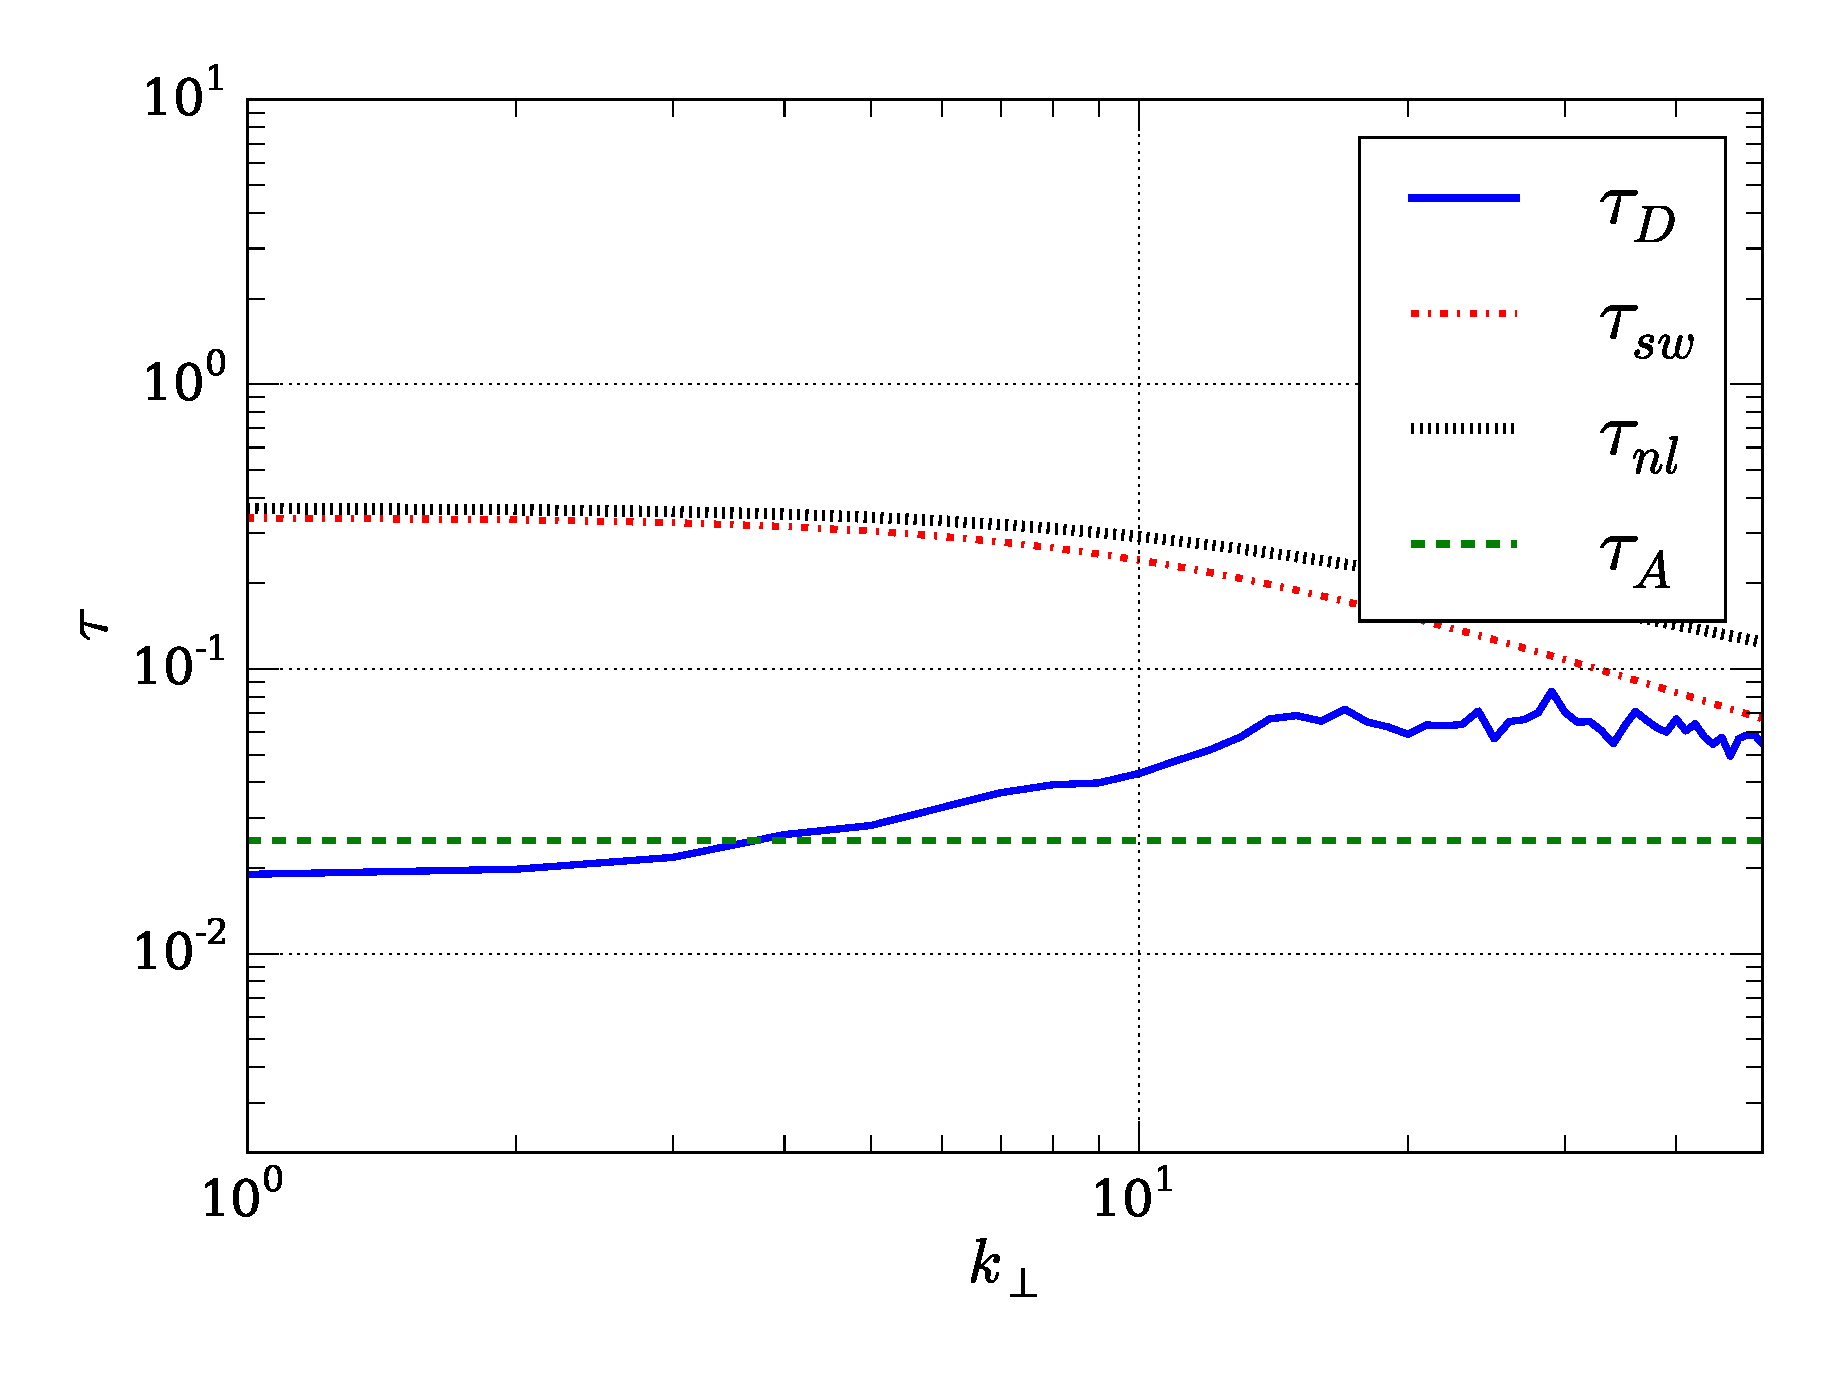
\includegraphics[width=0.76\columnwidth]{P1/fig5_B8_b_kpara_10.eps}
      \end{center}
    \end{minipage}
  \end{columns}
  \vspace{-0.5cm}
  \begin{center}
    $k_\parallel = 20$\\
    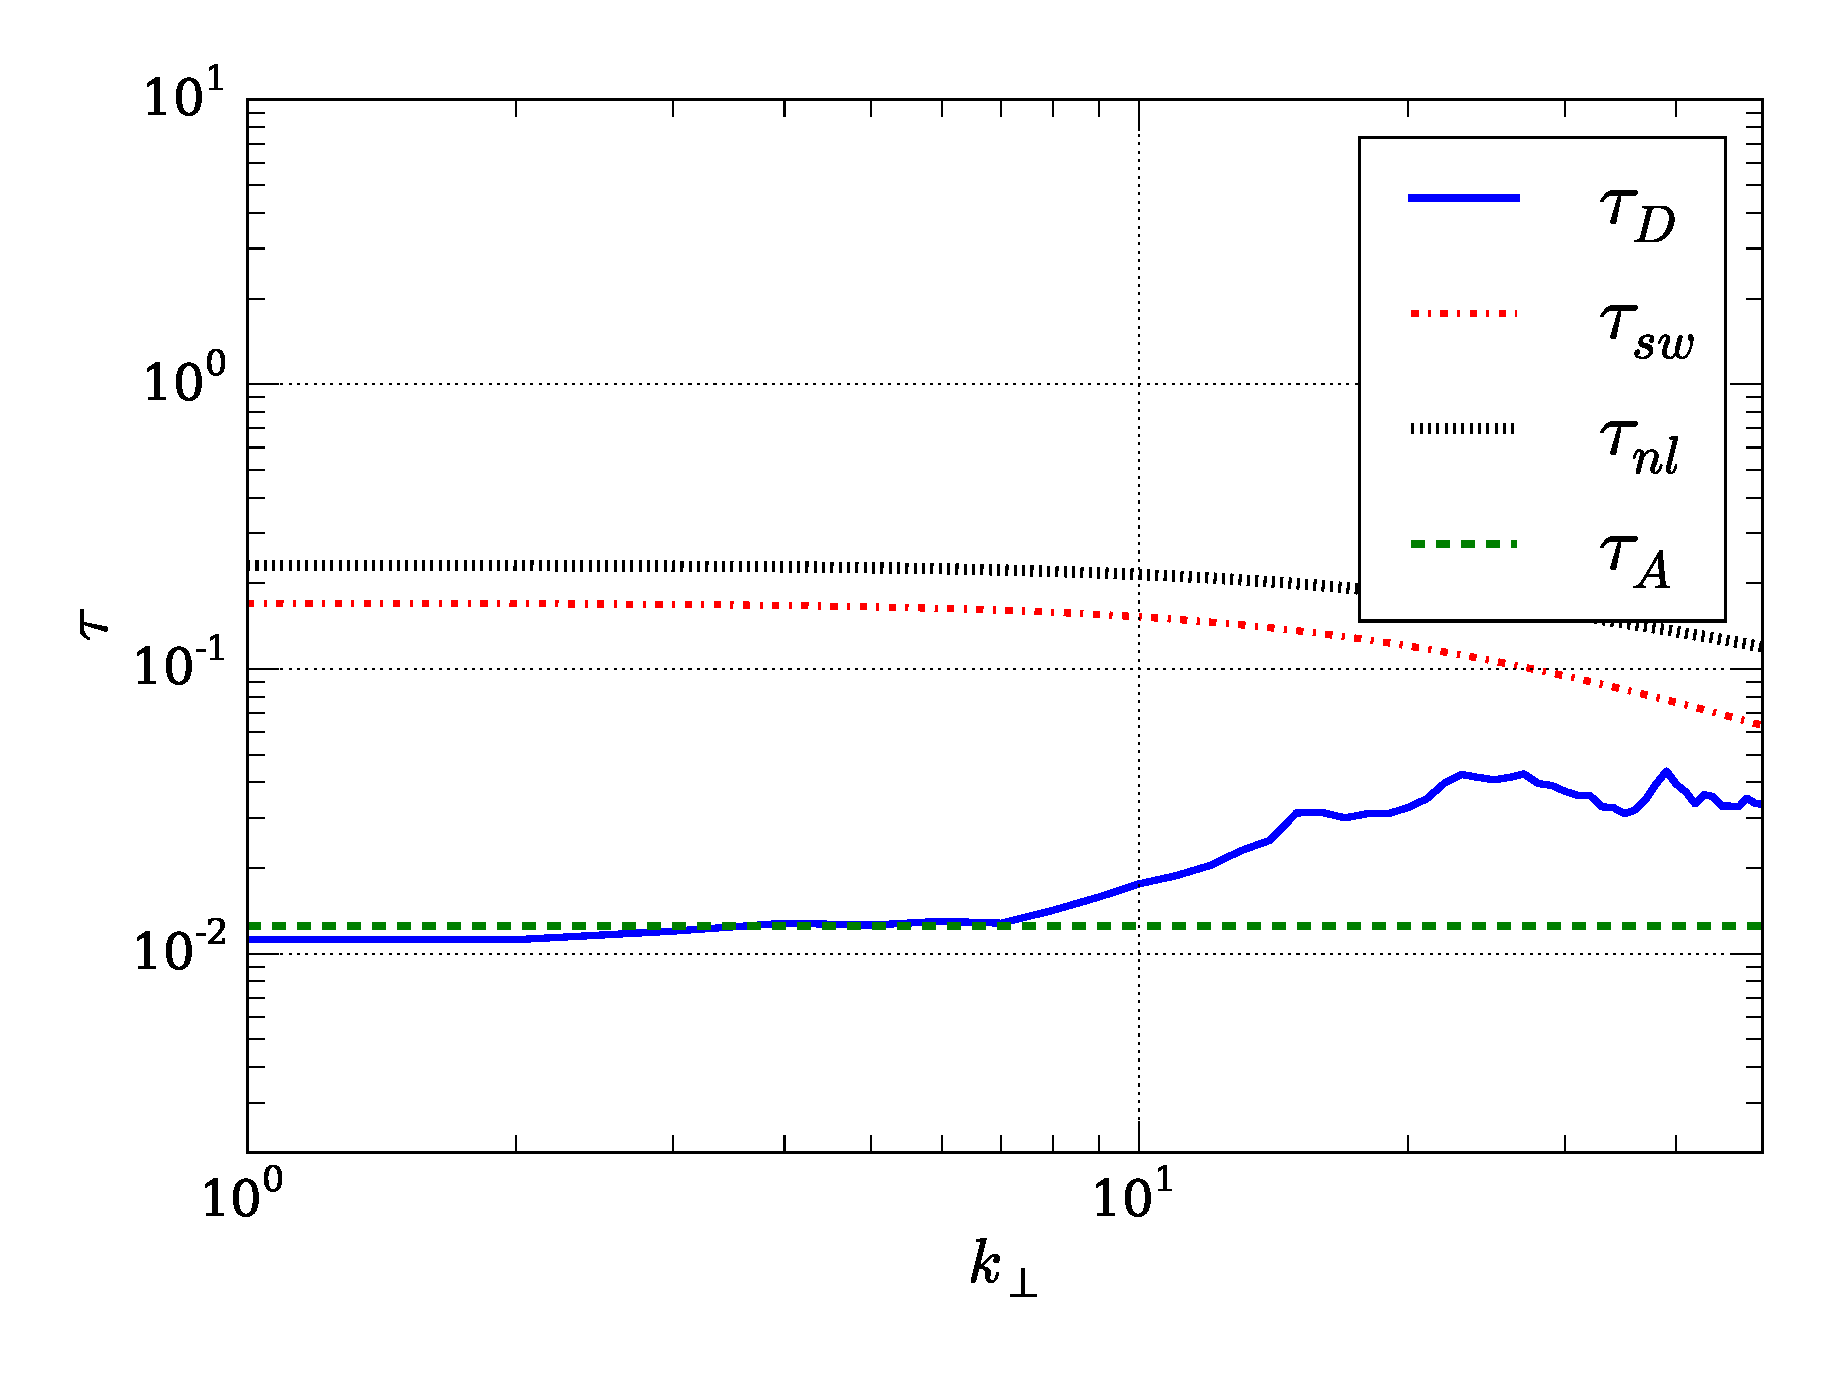
\includegraphics[width=0.38\columnwidth]{P1/fig5_B8_b_kpara_20.eps} \\
  \end{center}
}
\note[itemize]{
\item Para valores pequeños de $k_\perp$, el tiempo de Alfvén
  domina. Después, $\tau_D$ se acerca al \emph{sweeping}.
}


%\section{Conclusions}
\frame{\frametitle{Conclusiones hasta aquí...}
\pause
  \begin{itemize}
  \item Los efectos no locales (en el espacio espectral) juegan un rol
    importante en la turbulencia MHD y la descorrelación se encuentra
    principalmente dominada por el \emph{sweeping} y las interacciones
    Alfv\'enicas.
  \item El análisis presentado aquí permite \textbf{distinguir entre esos dos
    efectos}: las interacciones de \emph{sweeping} dominan la
    descorrelación para valores moderados de $B_0$, mientras que para
    grandes valores del campo medio $B_0$ y a grandes escalas las
    descorrelaciones están controladas mayoritariamente por las
    interacciones Alfv\'enicas.
  \item \textbf{El sistema elige el
    tiempo de descorrelación más corto disponible}. Aún
    para grandes valores del campo guía $B_0$, para escalas
    suficientemente pequeñas en las que el tiempo de \emph{sweeping}
    se vuelve más rápido que el tiempo de Alfv\'en, luego de un amplio
    rango de escalas dominadas por las ondas de Alfv\'en, el sistema
    transiciona hacia un comportamiento dominado por el
    \emph{sweeping}.
  \end{itemize}
}
\note[itemize]{
\item 2) SW+Alfvén confirma Servidio.
\item 3) Un constructo simple y relevante es que la tasa de
  descorrelación es la suman de las tasas asociadas con cada escala de
  tiempo relevante.
}


\frame{\frametitle{Conclusiones hasta aquí...}
  \begin{itemize}
  \item Extrapolación difícil de las conclusiones para aplicaciones
    espaciales y astrofísicas, pero sí resultados cualitativos.
  \item En MHD, tanto el \emph{sweeping} como la propagación de ondas
    de Alfv\'en contribuyen a la variación de tiempo total en un punto
    (espectro Euleriano en frecuencias), y por lo tanto influyen en
    una predicción limitante.
  \end{itemize}
}
\note[itemize]{
\item Por ejemplo, el viento solar admite $\delta B/B_0 \sim
    1$ en la escala más externa. Aún si el cociente es menor, por
    ejemplo a escalas menores en el rango inercial, el presente
    resultado sugiere que \textbf{el efecto de \textit{sweeping} se mantendría
    importante en establecer la tasa del tiempo de descorrelación en
    el ambiente interplanetario}.
\item
\item HELICIDAD CRUZADA
\item Para estudiar teniendo en cuenta el sentido de las propagaciónes, variables de Elsässer. Ahora el sentido de las propagaciones nos importa.

}



